% Journal version of the JCSS article; the rule-assembled attempt
% assembly-xdj406x0 stays the prespecified record (see README.md).
% The Springer Nature sn-jnl class and bibliography style are not
% redistributed here; build.py copies them from the local template folder.
% JCSS recommends the iicol option.
\documentclass[pdflatex,sn-mathphys-num,iicol]{sn-jnl}
\usepackage{amsmath,amssymb,xcolor}
\usepackage{graphicx}
\usepackage{array}
\usepackage{tikz}
\usetikzlibrary{arrows.meta,positioning,calc}
\usepackage{url}
\usepackage{xr-hyper}
\maxdeadcycles=1000
\newcommand{\bjtitle}[1]{\textit{#1}}
\newcommand{\bbtitle}[1]{\textit{#1}}
\newcommand{\burl}[1]{\url{#1}}
% Every result number is bound to values/result-values-final.json or
% values/journal-values.json; check.py verifies each binding.
\newcommand{\resultnum}[2]{#2}
\newcommand{\resultplural}[3]{#3}
\newcommand{\esmresource}{Online Resource~1}
\newcommand{\allunitsresource}{Online Resource~2}
\DeclareUrlCommand\code{\urlstyle{tt}\def\UrlBreaks{\do\_\do\.\do\:\do\/\do\-\do\|\do\,}}
% Import the other document's labels only after its caption macros exist.
\externaldocument[esm-]{esm}

\raggedbottom
\begin{document}

\title[Limits of detecting network influence]{Limits of Detecting Network Influence in Attitude Panels}

\author*[1]{\fnm{Davi} \sur{Abreu da Silveira}}\email{davi.silveira@sou.inteli.edu.br}

\author[1]{\fnm{Henrique Mohallem} \sur{Paiva}}\email{henrique@inteli.edu.br}

\affil*[1]{\orgname{Inteli -- Instituto de Tecnologia e Liderança}, \orgaddress{\city{São Paulo}, \state{SP}, \country{Brazil}}}

% The editorial office asked for each author's Google Scholar profile before
% the abstract (JCSO-D-26-00852, 31 October 2026).
\makeatletter
\let\jcss@printabstract\printabstract
\def\printabstract{{\addressfont Google Scholar profiles: Davi Abreu da Silveira, not available; Henrique Mohallem Paiva, \url{https://scholar.google.com/citations?user=BMHzItEAAAAJ}.\par}\vskip12pt\jcss@printabstract}
\makeatother

% \unboldmath: the class's author font sets \boldmath, which would leak
% into the abstract's math.
\abstract{\unboldmath Attitude panels record responses without observing social contacts, making network influence difficult to distinguish from individual persistence. We investigate the limits of this discrimination in a prespecified simulation with unobserved networks and explicit measurement error. Synthetic panels approximate the size and refreshment design of the Swiss Household Panel. A prespecified classifier compares their long-lag correlations with those of persistence models matched to short-term stability, while response reliability~$r$ is varied and known. Against trait-plus-autoregressive persistence, the estimated area under the receiver operating characteristic curve (AUC) first reached \resultnum{v4.protocol.target}{0.70} at $a=\resultnum{j.b.r055.first.point}{0.10}$ for $r=\resultnum{v4.tab.T1.B.r055.r}{0.55}$--\resultnum{v4.tab.T1.B.r090.r}{0.90} and at $a=\resultnum{j.b.r050.first.point}{0.30}$ for $r=\resultnum{v4.tab.T1.B.r050.r}{0.50}$; $a$ is the nominal fraction of innovation variance assigned to contacts. The prespecified comparison across persistence models was not interpretable under its eligibility rules. Subsequent exploratory analyses clarify the sensitivity of discrimination: a changing response channel separated panels without influence, while allowing persistence to fit reliability and one additional lag absorbed most separation by a lag-four-and-five classifier, with reliability shifts of only \resultnum{j.x3.free.r_shift.min}{0.0011}--\resultnum{j.x3.free.r_shift.max}{0.0028}. The study quantifies conditional detection limits and demonstrates their sensitivity to measurement and matching assumptions. Discriminating simulated panel distributions therefore requires separate justification before it can support attribution to social influence in observed panels.}

\keywords{Opinion dynamics, Social influence, Panel data, Measurement error, Model discrimination, Agent-based model}


\maketitle

\section{Introduction}\label{sec:intro}
% Every result number is bound; j.x2a.* and j.x5.* come from
% values/journal-transcribed.json, and j.x3.* from the tabulations of the
% released free-share catalog (rounds 4 and 5).
Opinion-dynamics models explain collective patterns through rules for how individuals revise their views in contact with others \cite{flache2017}; we use attitude and opinion interchangeably for those views. Recent work calibrates such models to individual transitions in panel surveys: Gestefeld and Lorenz fit a model with interpersonal updating to eleven annual waves of trust in government in the Swiss Household Panel (SHP) \cite{gestefeld2023}. Panels, however, record what people answer, not whom they talk to; the SHP observes no exposure beyond household co-residence. A model that reproduces short-term stability may fit for reasons unrelated to influence, so a calibration needs further evidence before its fit can count in favor of the interaction mechanism.

This article investigates the limits of discriminating network influence from individual persistence in attitude panels. The central issue is what a difference between their observed trajectories can establish when contacts are unobserved, measurement is imperfect and persistence can reproduce the same short-term stability. We quantify one aspect of that problem with a detection boundary: the nominal influence input at which a fixed classifier separates two specified panel distributions, as a function of response reliability. The boundary summarizes a conditional comparison; its meaning depends on the measurement assumptions and the persistence alternatives allowed.

The question is hard for two reasons. The first is measurement: a changed answer can reflect real change, a passing state or reporting error. Classical panel models separate the stability of a construct from the reliability of its measurement \cite{heise1969}, vague questions can make attitudes look more volatile than they are \cite{achen1975}, and updating between every wave may be hard to tell from settled dispositions measured with error \cite{kiley2020}. The second is identification. Observed behavior cannot reveal whether a group's average behavior affects its members unless reference groups are known \cite{manski1993}, and in observational network data contagion and homophily are generically confounded \cite{shalizi2011}. Without exposure data, influence from unobserved contacts and individual persistence can produce the same observed transitions; where they do not, the difference must appear somewhere in the trajectories.

Two analytic observations (Section~\ref{sec:methods-identification}) make the distinction concrete. Linear assimilation toward the population mean is observationally equivalent to individual autoregression matched at lag one: the population area under the receiver operating characteristic curve (AUC), the probability that a panel with influence is ranked above one without, is 0.5. For fixed random contacts, the influence term instead contains a contribution from the person's own state and an input from persistent contacts. The emphasis on the serial correlation of that input, and its possible role in discrimination, is an interpretation developed after the results became available.

% Design schematic (Fig. 1). Needs \usepackage{tikz} and
% \usetikzlibrary{arrows.meta,positioning,calc} in the preamble.
% The inset curve is a drawing, not data. Text sizes 7pt and 8pt bold use
% fonts already in the offline Tectonic cache.
\begin{figure*}[t]
\centering
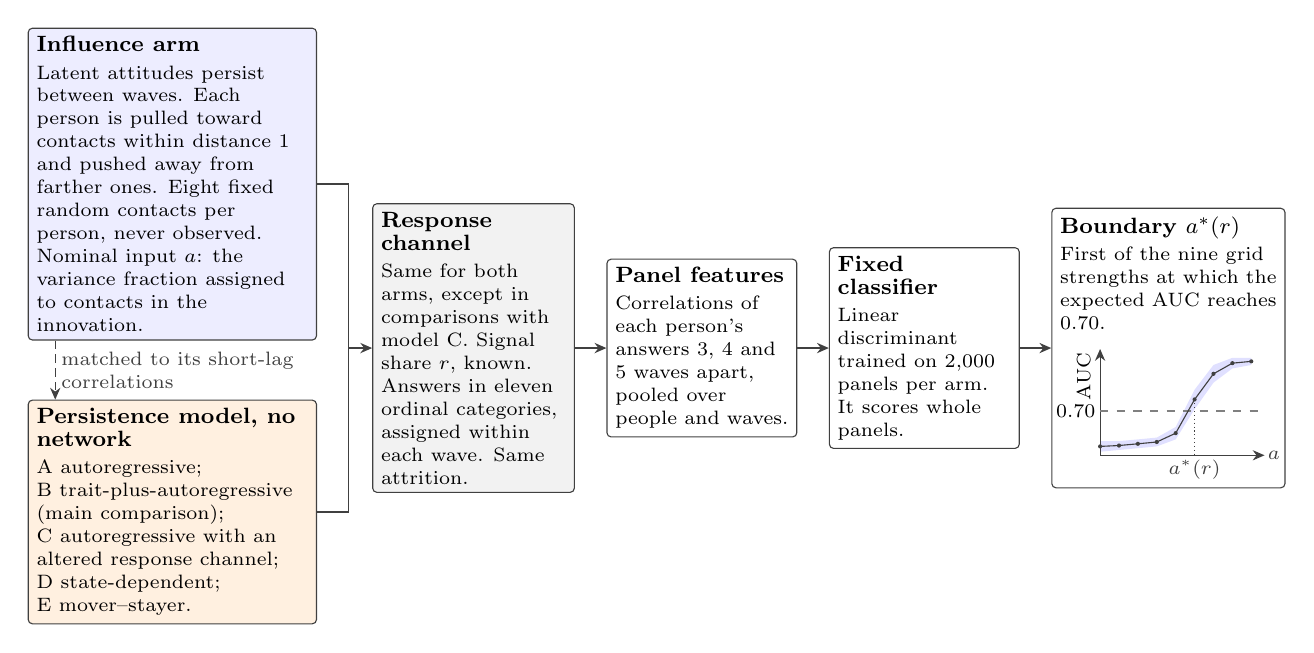
\begin{tikzpicture}[
  font=\fontsize{7pt}{8.3pt}\selectfont,
  >={Stealth[length=1.5mm,width=1.3mm]},
  box/.style={draw=darkgray, rounded corners=1.5pt, align=flush left,
    inner sep=3pt, text width=#1},
  box/.default=2.2cm,
  flow/.style={->, semithick, darkgray},
]
\node[box=3.45cm, fill=blue!7] (influence)
  {{\fontsize{8pt}{9.4pt}\selectfont\bfseries Influence arm}\\[1.5pt]
   Latent attitudes persist between waves. Each person is pulled toward
   contacts within distance~1 and pushed away from farther ones. Eight
   fixed random contacts per person, never observed. Nominal
   input~$a$: the variance fraction assigned to contacts in the innovation.};
\node[box=3.45cm, fill=orange!12, below=7.5mm of influence] (persistence)
  {{\fontsize{8pt}{9.4pt}\selectfont\bfseries Persistence model, no network}\\[1.5pt]
   A~autoregressive; B~trait-plus-autoregressive (main comparison);
   C~autoregressive with an altered response channel; D~state-dependent;
   E~mover--stayer.};
\draw[->, densely dashed, darkgray]
  ($(influence.south west)+(3.5mm,0)$) --
  node[right, align=flush left, inner sep=2pt] {matched to its short-lag\\
    correlations}
  ($(persistence.north west)+(3.5mm,0)$);

\coordinate (between) at ($(influence.east)!0.5!(persistence.east)$);
\node[box=2.35cm, fill=black!5, right=7mm of between] (channel)
  {{\fontsize{8pt}{9.4pt}\selectfont\bfseries Response channel}\\[1.5pt]
   Same for both arms, except in comparisons with model~C. Signal
   share~$r$, known. Answers in eleven ordinal categories, assigned within
   each wave. Same attrition.};
\coordinate (join) at ($(channel.west)+(-3mm,0)$);
\draw[semithick, darkgray] (influence.east) -| (join);
\draw[semithick, darkgray] (persistence.east) -| (join);
\draw[flow] (join) -- (channel.west);

\node[box, right=4mm of channel] (features)
  {{\fontsize{8pt}{9.4pt}\selectfont\bfseries Panel features}\\[1.5pt]
   Correlations of each person's answers 3, 4 and 5 waves apart, pooled
   over people and waves.};
\node[box, right=4mm of features] (classifier)
  {{\fontsize{8pt}{9.4pt}\selectfont\bfseries Fixed classifier}\\[1.5pt]
   Linear discriminant trained on 2,000 panels per arm. It scores whole
   panels.};
\draw[flow] (channel) -- (features);
\draw[flow] (features) -- (classifier);

\node[box=2.75cm, right=4mm of classifier, minimum height=3.55cm]
  (boundary) {};
\node[anchor=north west, inner sep=3pt, text width=2.75cm,
  align=flush left] at (boundary.north west)
  {{\fontsize{8pt}{9.4pt}\selectfont\bfseries Boundary $a^*(r)$}\\[1.5pt]
   First of the nine grid strengths at which the expected AUC
   reaches 0.70.};
\draw[flow] (classifier) -- (boundary);
% Inset drawn in centimeters; the AUC axis runs from 0.45 at the origin.
\begin{scope}[shift={($(boundary.south west)+(0.62cm,0.42cm)$)}]
  \fill[blue!12] (0.000cm,0.045cm) -- (0.240cm,0.068cm) -- (0.480cm,0.090cm) -- (0.720cm,0.113cm) -- (0.960cm,0.202cm) -- (1.200cm,0.585cm) -- (1.440cm,0.922cm) -- (1.680cm,1.103cm) -- (1.920cm,1.147cm) -- (1.920cm,1.238cm) -- (1.680cm,1.238cm) -- (1.440cm,1.147cm) -- (1.200cm,0.833cm) -- (0.960cm,0.360cm) -- (0.720cm,0.225cm) -- (0.480cm,0.202cm) -- (0.240cm,0.180cm) -- (0.000cm,0.180cm) -- cycle;
  \draw[->, darkgray] (0cm,0cm) -- (2.088cm,0.000cm) node[right, inner sep=1pt] {$a$};
  \draw[->, darkgray] (0cm,0cm) -- (0.000cm,1.350cm);
  \node[rotate=90, anchor=south, inner sep=1pt] at (-0.08cm,1.0cm) {AUC};
  \draw[dashed, gray] (0.000cm,0.562cm) -- (2.040cm,0.562cm);
  \node[left, inner sep=1.5pt] at (0.000cm,0.562cm) {0.70};
  \draw[darkgray] (0.000cm,0.113cm) -- (0.240cm,0.124cm) -- (0.480cm,0.146cm) -- (0.720cm,0.169cm) -- (0.960cm,0.281cm) -- (1.200cm,0.709cm) -- (1.440cm,1.035cm) -- (1.680cm,1.170cm) -- (1.920cm,1.193cm);
  \fill[darkgray] (0.000cm,0.113cm) circle (0.75pt);
  \fill[darkgray] (0.240cm,0.124cm) circle (0.75pt);
  \fill[darkgray] (0.480cm,0.146cm) circle (0.75pt);
  \fill[darkgray] (0.720cm,0.169cm) circle (0.75pt);
  \fill[darkgray] (0.960cm,0.281cm) circle (0.75pt);
  \fill[darkgray] (1.200cm,0.709cm) circle (0.75pt);
  \fill[darkgray] (1.440cm,1.035cm) circle (0.75pt);
  \fill[darkgray] (1.680cm,1.170cm) circle (0.75pt);
  \fill[darkgray] (1.920cm,1.193cm) circle (0.75pt);
  \draw[densely dotted, darkgray] (1.200cm,0.709cm) -- (1.200cm,0.000cm)
    node[below, inner sep=1.5pt] {$a^*(r)$};
\end{scope}
\end{tikzpicture}
\caption{Design of the simulation. At each signal share $r$ and influence
strength $a$, panels from the influence arm and from a persistence model
matched to its short-lag correlations pass through the same response channel
(model C alters it in the persistence arm). A fixed classifier scores whole
panels from their long-lag correlations. The boundary $a^*(r)$ is the first
of the nine grid strengths at which the expected AUC reaches 0.70; the shaded area stands for the simultaneous uncertainty
band. Matching, training and testing use separate simulated panels. The inset
is a drawing, not data. \esmresource, Table~\ref{esm-tab:glossary-terms}, defines
the terms used in the article.}
\label{fig:design}
\end{figure*}


We study these limits in a prespecified simulation in which the generating mechanism is known (Fig.~\ref{fig:design}). Synthetic eleven-wave panels approximate the size and refreshment design of the SHP trust series. In the influence arm, persistent latent attitudes are pulled toward similar contacts and pushed away from dissimilar ones on an unobserved random network. The parameter $a$ sets the nominal fraction of innovation variance assigned to contacts; it is neither the realized fraction of attitude change attributable to them nor a directly interpretable measure of social influence in a survey. Five persistence alternatives are matched to short-lag population correlations. The response channel has known signal share $r$, its reliability before discretization. A fixed linear classifier scores whole panels from their pooled correlations three to five waves apart, and $a^*(r)$ is the first grid strength at which the expected AUC reaches \resultnum{v4.protocol.target}{0.70}.

The contribution is a quantitative account of the conditions under which such discrimination is informative and where it breaks down. The design separates successful comparisons from failures to fit or validate, rather than treating a failed alternative as evidence for influence. It also distinguishes the prespecified results from later exploratory analyses that examine how the result changes when measurement and persistence assumptions are relaxed. The protocol was adopted after partial exposure to calibration results, and the confirmatory run used new seeds; the study is prespecified rather than publicly registered (Section~\ref{sec:methods-record}).

Against trait-plus-autoregressive persistence, the estimated AUC first reached \resultnum{v4.protocol.target}{0.70} at $a=\resultnum{j.b.r055.first.point}{0.10}$ for every signal share from \resultnum{v4.tab.T1.B.r055.r}{0.55} to \resultnum{v4.tab.T1.B.r090.r}{0.90} and at $a=\resultnum{j.b.r050.first.point}{0.30}$ for $r=\resultnum{v4.tab.T1.B.r050.r}{0.50}$. Under an equal-variance normal approximation at a one-sided 5\% level, an AUC of 0.70 gives a test on a single panel a power of about \resultnum{j.auc_translation.target070.power}{0.18} against a known persistence score distribution.

These confirmatory findings establish discrimination against the main persistence alternative under favorable measurement assumptions. The prespecified comparison across all persistence models could not be interpreted, because the altered response channel failed the zero-strength validity rule and the declared solver did not obtain acceptable state-dependent fits near the main boundary. The exploratory analyses then show why the main result is sensitive to the comparison design. A changing response channel separated panels without influence, while allowing persistence to fit reliability and an additional lag absorbed most separation by a classifier using the remaining lags. The fitted reliability differed from the design value by only \resultnum{j.x3.free.r_shift.min}{0.0011}--\resultnum{j.x3.free.r_shift.max}{0.0028}; this combined change does not isolate the effect of reliability alone.

The resulting distinction between discrimination and attribution is consequential for models calibrated to attitude panels \cite{manski1993,shalizi2011,cohencole2008}. The Discussion examines three limits: the restricted persistence alternatives, privileged knowledge of reliability and the absence of network burn-in. It separates sensitivities demonstrated by the exploratory analyses from the untested effects of richer persistence and initial transients, and considers what additional evidence would make an influence interpretation more credible (Section~\ref{sec:implications}).


\section{Theoretical background and related work}\label{sec:background}
% Sources and the claim checked for each citation are recorded in
% literature-verification.md in this directory.
\subsection{Opinion dynamics and validation against survey data}\label{sec:bg-opinion}

Flache and colleagues distinguish assimilative influence, which reduces differences between connected agents; similarity-biased influence, which limits assimilation to agents who are already close; and repulsive influence, which can widen differences after contact \cite{flache2017}. Classic models average the opinions of contacts \cite{degroot1974}, keep an anchor to initial opinions \cite{friedkin1990}, or let agents compromise only with others within a confidence bound, in random pairs \cite{deffuant2000} or with all such neighbors at once \cite{hegselmann2002}; repulsive variants move agents away from sources that are too dissimilar \cite{jager2005}. Evidence for these shapes is mixed. Tak\'acs, Flache and M\"as found no support for the idea that discrepancy or disliking pushes opinions away from the source; shifts toward the source grew with opinion distance \cite{takacs2016}, which also speaks against a confidence bound. In field data on adolescents, a stochastic actor-oriented model found negative influence, but little support for bounded confidence, in preferences for one clothing style \cite{tang2025empirical}.

Many such models are judged by aggregate patterns, such as the segregated communities that a model of influence and unfollowing produced, consistent with Twitter data \cite{sasahara2021}. Answering calls for empirical tests of micro-level assumptions \cite{flache2017}, Gestefeld and Lorenz calibrate an interaction model to institutional-trust distributions from the European Social Survey and to annual trust transitions of SHP respondents \cite{gestefeld2023}. With repeated surveys and recorded communication among the same people, Nurek and colleagues find that a baseline in which everyone keeps their opinion reaches a high overall F1 score while detecting no change, and that on real-world data opinion-dynamics models often fail to outperform such trivial baselines \cite{coding2024}. Moor-Smith and Carpentras show with synthetic data that even the generating model, rerun with its true parameters, beats a no-change baseline only above a minimum amount of opinion change, and that where the signal is weak the calibrated model learns to mimic that baseline and ``freeze'' \cite{moor2026}. Random noise and scale distortions, unlike binning, strongly affect the predictions of the Deffuant model \cite{carpentras2022}, and monotone distortions of the scale can make data generated by that model look incompatible with it \cite{carpentras2023}. In the terms of pattern-oriented modeling \cite{grimm2005}, our design treats short-lag correlations as the pattern that competing processes must share and longer-lag correlations as the pattern that may tell them apart.

\subsection{Measurement error, stability and state dependence}\label{sec:bg-measurement}

Unstable answers have long been read in two ways. Converse's ``black-and-white'' model divided respondents into stable opinion holders and unstable changers whose answers are essentially random \cite{converse1964}; Achen attributed nearly all of the apparent inconsistency to vague questions and response categories \cite{achen1975}. Zaller and Feldman proposed that most people answer with whatever ideas are at the top of their heads \cite{zaller1992}, and averaging many items on the same issue removes much of the measurement error and reveals stable preferences \cite{ansolabehere2008}. In a four-wave Swiss panel, Hill and Kriesi \cite{hill2001,hillkriesi2001} added a group of durable changers to Converse's two groups, with results that undermine the measurement-error model. Reliability varies widely across items \cite{alwin2007,alwinkrosnick1991reliability}: of 293 core items of the General Social Survey, 133 had reliabilities above 0.70 and 15 fell below 0.40 \cite{hout2016}, and the average measurement quality of 67 European Social Survey questions ranges from 0.25 to 0.88 \cite{poses2021}.

Trait--state--error models \cite{kenny1995tse} add a stable trait to the classical panel models of stability and reliability \cite{heise1969,wiley1970}, but they often give improper or unstable estimates, especially when waves are few \cite{cole2005tso,ludtke2018starts}. Ignoring the trait has its own cost: under realistic assumptions the cross-lagged panel model is very likely to find spurious cross-lagged effects \cite{lucas2023,hamaker2015critique}, which is why trait-plus-autoregressive persistence (model B) is the main comparison here. In General Social Survey panels, most change looks like short-term change or measurement error \cite{kiley2020,vaiseykiley2021}, while in six long household panels, the SHP among them, persistent change over the life course accompanies substantial year-to-year fluctuation \cite{lersch2023}.

In economics and statistics the same problem appears as state dependence versus heterogeneity. Heckman distinguishes true state dependence, in which experience changes later choices, from spurious state dependence, in which past outcomes predict future ones only because they proxy for persistent unobserved differences \cite{heckman1981}. Earlier, Feller pointed out that the same distribution of event counts arises from contagion and from heterogeneity, so that deciding between them requires the correlation between time intervals, not the distribution alone \cite{feller1943}. Mover--stayer models mix people who never change category with people who move as a Markov chain \cite{blumen1955,goodman1961}. Persistence can also differ between people, as when the stability of party identification rises with age \cite{alwinkrosnick1991}, and sums of simple series, including a series measured with error, typically follow mixed autoregressive moving-average models \cite{granger1976}. Our persistence models cover autoregressive, trait, state-dependent and mover--stayer forms, but not several autoregressive speeds or speeds that vary between people.

\subsection{Identifying social influence}\label{sec:bg-identification}

Manski's identification problem does not vanish when reference groups are known: inference is then difficult or impossible if the variables that define groups and those that directly affect behavior are functionally dependent or statistically independent \cite{manski1993}. When interactions follow a known social network, endogenous and exogenous peer effects in an extended linear-in-means model are generally identified, although identification can fail for particular network structures \cite{bramoulle2009}.

Observational studies face a second confound: people form ties with similar others \cite{mcpherson2001}. Christakis and Fowler reported that obesity appears to spread through social ties \cite{christakis2007}; with the same kind of models, Cohen-Cole and Fletcher found ``network effects'' for acne, headaches and height that became smaller and insignificant after adjustment for environmental confounders \cite{cohencole2008}; matched-sample estimation attributed more than half of the apparent contagion in product adoption to homophily \cite{aral2009}, and sensitivity analysis asks how strong latent homophily or confounding would have to be to explain away a contagion effect \cite{vanderweele2011}. When ties and behavior are observed over several waves, stochastic actor-oriented models separate selection from influence \cite{snijders2010,steglich2010}, and simulations with known truth have tested estimators of influence and selection \cite{zachrison2016,daza2021}. Other work treats measurement error as error in the observed network rather than in the responses \cite{xu2021sensitivity,advani2018credibly}.

Some recent methods dispense with observed links, identifying linear network models from many separate networks with known membership \cite{lewbel2023} or from panels with many periods relative to the number of ties per unit \cite{depaula2024}, or inferring the network and the interaction kernel jointly from multiple trajectories \cite{lang2026joint}. None of these routes fits the panels studied here: each is a single realization with eleven waves, thousands of respondents and no known groups, and the influence rule is nonlinear.

Even with observed networks, influence is hard to detect: in simulated friendship networks with three-category opinions, a stochastic actor-oriented model detected an influence effect of 0.8 in 10\% of 200 data sets with two waves and 30 actors, against 97.5\% with five waves and 120 actors \cite{stadtfeld2020}.

\subsection{Simulation-based model discrimination}\label{sec:bg-discrimination}

The criterion used here is a classifier two-sample comparison. If two samples share a distribution, a classifier trained to tell them apart should stay near chance on held-out data; statistically significant accuracy above chance indicates that they differ in a way the classifier can use \cite{lopezpaz2017}. Such tests are consistent whenever the classifier's true accuracy stays bounded away from chance, and in a high-dimensional Gaussian setting a linear-discriminant test loses only a constant factor of efficiency relative to Hotelling's test \cite{kim2021classifier}. A classifier that sees a few summary statistics can still miss differences: in approximate Bayesian computation, model choice based on insufficient summaries can be unreliable \cite{robert2011}. Our persistence models are fitted by matching moments of simulated panels, in the spirit of indirect inference \cite{gourieroux1993}.

Two further results bound what such comparisons can show. Gelastopoulos, Sage and van de Rijt prove that the joint distribution of any stochastic process describing longitudinal observations can be reproduced exactly both by a pure reinforcement model, driven by past observations and independent noise, and by a pure heterogeneity model, driven by a fixed latent variable and noise \cite{gelastopoulos2025}. With functional forms left unrestricted, the theorem guarantees that a twin exists, not that a given parametric family can serve as one. In a preprint, Ure\~{n}a-Carrion, Peixoto and I\~{n}iguez show that likelihood-based selection among binary spreading mechanisms on known, fully observed networks can fail under common conditions \cite{urena2026}. A boundary against fixed persistence models matched at most at lags one and two is therefore a finite contrast that does not contradict generic equivalence.

\subsection{Positioning}\label{sec:bg-positioning}

Table~\ref{tab:positioning} compares the design with its closest antecedents. In the table, the studies that observe networks or communication do not model response error, the panel studies that model response error contain no influence between people, and the studies that fit influence models to survey data judge them by fit or against simple baselines, not against persistence matched to the same short-term stability. No single component is new; to our knowledge, based on a documented but limited search (\esmresource, Section~\ref{esm-sec:search}), the combination is.

% Two-column float with the structure of the class's table environment
% (8 bp body font, notes under the tabular), which table* lacks.
\begin{table*}[tp]
\begin{center}
\begin{threeparttable}
\tablebodyfont
\caption{Closest antecedents and the present design}\label{tab:positioning}
\setlength{\tabcolsep}{3pt}
\begin{tabular}{@{}p{0.17\textwidth}lllllp{0.21\textwidth}@{}}
\toprule
\raggedright Study & \begin{tabular}[t]{@{}l@{}}Network\\observed\end{tabular} & \begin{tabular}[t]{@{}l@{}}Exposure\\measured\end{tabular} & \begin{tabular}[t]{@{}l@{}}Response\\error\\modeled\end{tabular} & \begin{tabular}[t]{@{}l@{}}Individual\\trajectories\end{tabular} & \begin{tabular}[t]{@{}l@{}}Matched\\no-network\\persistence\end{tabular} & \raggedright Criterion\tabularnewline
\midrule
\raggedright Gestefeld and Lorenz \cite{gestefeld2023} & No & No & No & Partly$^{a}$ & No & \raggedright Fit to distributions and transition matrices\tabularnewline
\raggedright Nurek et al.\ \cite{coding2024} & Yes & Yes$^{b}$ & No & Yes & No$^{c}$ & \raggedright F1 and divergence against simple baselines\tabularnewline
\raggedright Moor-Smith and Carpentras \cite{moor2026} & No & No & No$^{d}$ & No$^{e}$ & No$^{c}$ & \raggedright Variance explained beyond no change\tabularnewline
\raggedright Kiley and Vaisey \cite{kiley2020} & No & No & Partly$^{f}$ & Yes & n/a$^{f}$ & \raggedright BIC of updating versus settled models\tabularnewline
\raggedright Mulder \cite{mulder2023}; Dang and Ma \cite{dang2026}, preprint & No & No & Yes & Yes & n/a$^{g}$ & \raggedright Power of a test of a within-person cross-lagged effect\tabularnewline
\raggedright Stadtfeld et al.\ \cite{stadtfeld2020} & Yes & Yes & No & Yes & No$^{h}$ & \raggedright Power of a test of the influence parameter\tabularnewline
\raggedright Ure\~{n}a-Carrion et al.\ \cite{urena2026}, preprint & Yes & Yes & No & Yes & No$^{i}$ & \raggedright Likelihood-based model selection\tabularnewline
\raggedright This study & No & No & Yes$^{j}$ & Yes & Yes$^{k}$ & \raggedright AUC of a fixed LDA on pooled lag-3--5 correlations\tabularnewline
\botrule
\end{tabular}
\par\vskip3pt\tablefootnotefont Network observed: ties among respondents are known. Exposure measured: what contacts say or do is recorded. Matched no-network persistence: a persistence process without a network, fitted to the same short-lag correlations. $^{a}$Transitions between consecutive annual waves. $^{b}$Communication events and survey opinions are observed; the opinion expressed in each event is simulated. $^{c}$Compared with simple baselines, such as unchanged opinions. $^{d}$Noise is added to the opinion process, not to responses. $^{e}$Repeated cross-sections. $^{f}$No influence model; settled dispositions and active updating are compared, and deviations from a settled disposition absorb measurement error together with short-lived change. $^{g}$No influence between people; the null is a zero within-person cross-lagged effect. $^{h}$Test of the influence parameter against zero in the same model. $^{i}$An independent spreading mechanism is among the candidate models. $^{j}$Known signal share $r$; eleven ordinal categories. $^{k}$Matched at lag one, or at lags one and two. BIC, Bayesian information criterion; AUC, area under the receiver operating characteristic curve; LDA, linear discriminant analysis.\par
\end{threeparttable}
\end{center}
\end{table*}


\section{Materials and methods}\label{sec:methods}
% Technical passages cut from the rule-assembled Methods are kept in
% esm/design-details.tex (Online Resource 1, Section S3). Unbound numbers in
% this file are design constants or analytic values of the frozen kernel, not
% results.
\subsection{Synthetic panels and network influence}\label{sec:methods-panels}

Each synthetic panel (Fig.~\ref{fig:design}) follows 10,626 people in two-person households over eleven annual waves ($t=0,\ldots,10$): 7,084 enter at $t=0$ and 3,542 at $t=5$ as a refreshment sample. Households stay from one wave to the next with probability 0.89, independently of attitudes. This approximates the size of the SHP trust series analyzed by Gestefeld and Lorenz \cite{gestefeld2023} and the SHP's refreshment design \cite{voorpostel2025shp}, not its observed counts, persistence or selective attrition \cite{lipps2007,voorpostel2010}. In the SHP, co-residents aged 14 and older answer individual questionnaires \cite{voorpostel2025shp} and form a partially observed dyadic exposure of the kind that actor--partner models use \cite{kennykashy2006,kim2024}; our synthetic households carry no attitude coupling.

In the influence arm, each person $i$ has a latent attitude $z_{it}$ on a standard-normal scale and eight contacts drawn at random once per panel; the network never changes, and the analysis never sees it. The influence term averages a distance-dependent kernel over the contacts,
\begin{equation}
\begin{aligned}
D_{it}&=\frac18\sum_{j\in\mathcal N_i}f(z_{jt}-z_{it}),\\
f(g)&=\begin{cases}g,&|g|\le1,\\-b\,g,&|g|>1,\end{cases}
\end{aligned}
\end{equation}
with $b=0.25$: people are pulled toward contacts within distance one and pushed weakly away from farther ones, an assimilation--contrast shape like that of bounded-confidence models with repulsion \cite{flache2017,jager2005}. The term is standardized across the population to $d_{it}$, and
\begin{equation}
\begin{aligned}
h_{i,t+1}&=0.85\,z_{it}+\sqrt{1-0.85^2}\,\bigl(\sqrt a\,d_{it}\\
&\qquad+\sqrt{1-a}\,\xi_{it}\bigr),\\
\mathbf z_{t+1}&=R_N(\mathbf h_{t+1}),
\end{aligned}
\end{equation}
where $\xi_{it}$ is standard-normal noise and the rank transport $R_N$ replaces the updated values by fixed normal quantiles in the same order.

The influence strength $a$ is the nominal fraction of innovation variance assigned to contacts, not a realized or causal share of attitude change, and is not comparable with the parameters of standard opinion models. An exploratory analysis measures the drift term's partial $R^2$ for the next latent attitude beyond linear persistence (Section~\ref{sec:results-exploratory}). Because $R_N$ restores the same distribution at every step, the process cannot produce clustering or polarization in the population marginal; this does not exclude dependence between connected individuals. It retains the local shape of the kernel as a test bed for detection, not a model of how trust evolves. Panels start without burn-in from states unrelated to the network, so the dependence between people and their contacts builds up during the observed waves, and this start-up adjustment is part of what can be detected. There is one update per wave, and $a$ takes the values $G=\{0,0.001,0.003,0.01,0.03,0.10,0.30,0.60,0.90\}$.

\subsection{Persistence models and matching}\label{sec:methods-persistence}

The persistence arm has no network. Its five alternatives use the same rank transport: autoregressive persistence (A); a stable individual trait plus autoregression (B, the main comparison); autoregression with an altered response channel (C); state-dependent persistence, with greater stability at extreme attitudes (D); and mover--stayer persistence, with a subgroup fixed at its initial position (E). Their equations and parameter boxes are in \esmresource, Sections~\ref{esm-sec:dd-channels} and~\ref{esm-sec:dd-matching}.

At $a=0$ the influence arm is model A with $\phi=0.85$, and with $\lambda=\pi=\gamma=0$ models A, B, D and E coincide exactly with it when they share random numbers, so their comparison at zero strength is an identity, a property of the simulator rather than evidence that social mechanisms are identifiable; model C lacks this identity, because only its arm receives the altered channel.

Each persistence model is matched at the same $(a,r)$ on within-person correlations of answers one wave apart (A and C) or one and two waves apart (B, D and E), pooled over people and waves and averaged over many simulated panels. Fits must meet the prespecified numerical tolerance and pass validation on fresh panel pairs. The sample sizes, solver, retry and acceptance rules are in \esmresource, Section~\ref{esm-sec:dd-matching}. A failed fit at one $(a,r)$ is a gap, recorded by reason and never treated as evidence of discrimination. Reported family limits concern the operational feasibility screen or the declared solver and parameter box; they do not prove that the broader persistence family cannot match (\esmresource, Section~\ref{esm-sec:dd-feasibility}).

\subsection{Response channel}\label{sec:methods-channel}

Both arms are observed through the same response channel, $w_{it}=\sqrt r\,z_{it}+\sqrt{1-r}\,e_{it}$, with standard-normal response error $e_{it}$. The signal share $r$ is the latent state's share of variance in this continuous response before discretization, that is, its reliability. It is a design parameter known to both arms, not an estimate for a survey item; reliability estimates cannot be transferred between items, wordings, countries and models without validation \cite{antoun2026,lucasdonnellan2012,alwinkrosnick1991reliability}. We use $r\in\{0.50,0.55,\ldots,0.90\}$; $r=0.70$ was examined during the calibration that preceded the frozen protocol and is marked $\dagger$ in tables. In each wave, the respondents' continuous responses are ranked and allocated to eleven approximately equiprobable categories, 0 to 10, so both arms have the same category distribution in every wave and shifts in the response margins are removed; temporal dependence can still vary.

In comparisons with model C, only the persistence arm receives response error that is larger near the center of the scale and heaping at the center with probability 0.10. Secondary channels add persistent response style, a signal share that rises with earlier interviews (a stand-in for panel conditioning), and error-free and rank-based versions of the responses (\esmresource, Section~\ref{esm-sec:dd-channels}).

\subsection{Classifier, criterion and boundaries}\label{sec:methods-classifier}

The classifier scores whole panels from the pooled within-person correlations of answers three, four and five waves apart, $L_3$, $L_4$ and $L_5$, treating categories as equally spaced scores. The linear-discriminant specification is fixed, but a separate rule is trained for each comparison, strength and signal share, using panels separate from evaluation and without threshold or tuning search. Its standardization, covariance regularization and sample sizes are specified in \esmresource, Section~\ref{esm-sec:dd-classifier}. For a given matched model and trained rule, AUC is the probability that a new influence panel receives a higher score than a new persistence panel, counting ties as half.

Let $\mathcal A(a,r)$ be the population AUC for new panels from the two laws, averaged over the prespecified matching, validation and training procedure and conditional on a successful fit. The first boundary is
\begin{equation}
a^*(r)=\min\{a\in G:\mathcal A(a,r)\ge0.70\},
\end{equation}
estimated as the lowest grid strength whose point AUC reaches 0.70, or not attained if none does on a complete grid; a sustained boundary $a^*_s(r)$, from which the AUC stays at or above 0.70 at every higher strength, guards against a curve that falls back. The primary estimand is the whole curve $a^*(r)$ against model B; targets 0.60 and 0.80 are secondary. An AUC of 0.70 is often read as the lower end of acceptable discrimination \cite{hosmer2013}, but the protocol records no reason for this target, for the shrinkage of the discriminant or for the parameter box, all inherited conventions (\esmresource, Table~\ref{esm-tab:design-conventions}).

\begin{table}[t]
\caption{Normal-theory translation of the AUC targets into the power of a test on one panel}\label{tab:auc-translation}
\begin{tabular}{@{}lll@{}}
\toprule
AUC target & $\delta$ (score SDs) & Power, one panel \\
\midrule
\resultnum{j.target.r060}{0.60} (secondary) & \resultnum{j.auc_translation.target060.delta}{0.36} & \resultnum{j.auc_translation.target060.power}{0.10} \\
\resultnum{j.target.r070}{0.70} (primary) & \resultnum{j.auc_translation.target070.delta}{0.74} & \resultnum{j.auc_translation.target070.power}{0.18} \\
\resultnum{j.target.r080}{0.80} (secondary) & \resultnum{j.auc_translation.target080.delta}{1.19} & \resultnum{j.auc_translation.target080.power}{0.32} \\
\botrule
\end{tabular}
\end{table}

Table~\ref{tab:auc-translation} translates AUC into the power of a one-panel test against a known persistence score distribution, under an equal-variance normal approximation. It is an illustration of practical discrimination, not a measured rejection rate or a test available for an observed survey without further assumptions; the formula is in \esmresource, Section~\ref{esm-sec:dd-classifier}.

Approximate nominal 95\% bands combine network-cluster resampling with local propagation of matching and training uncertainty. They are simultaneous over the available strengths of one comparison at one signal share, not over all comparisons or reliabilities; their construction and inversion are in \esmresource, Section~\ref{esm-sec:dd-band}. The grid is coarse above 0.10: $a^*(r)=0.10$ means that no lower grid strength attained the target, not that a continuous threshold was estimated. No interpolation, smoothing or monotonicity constraint is imposed.

One comparison at one signal share forms a unit, valid if its zero-strength cell was fitted with a band containing 0.5 and otherwise complete but invalid, with its boundaries suppressed. The main curve is valid only if all nine units against B are complete and valid; a reading across persistence models also required every unit of models A, C, D and E to be complete and valid. Gaps censor rather than invalidate: no boundary is declared across a gap (\esmresource, Section~\ref{esm-sec:dd-band}).

\subsection{What separates the arms}\label{sec:methods-identification}

Two analytic observations frame what the classifier can find. First, if each person were instead pulled linearly toward the population mean, the influence term would be proportional to the person's own state, because transport fixes the mean at zero. The update would remain an autoregression, model A matched at lag one would have exactly the same law, and the population AUC would be 0.5 for any classifier.

Second, treating random contacts as independent of the person's own state gives a first-order decomposition into an own-state conditional mean and a deviation contributed by the particular contacts (\esmresource, Section~\ref{esm-supp:drift-mean}). Because those contacts are fixed and their attitudes persist, their contribution is serially correlated. Even linear averaging over fixed contacts, as in DeGroot's model \cite{degroot1974}, can generate such an input. No tested persistence model contains that component. The classifier observes only pooled lag correlations, so it cannot attribute their differences specifically to contact between people. The possible role of this correlated input in the observed separation is an interpretation developed after the results, not a tested explanation.

The estimand also uses privileged information: both arms share known reliability, and matching targets population moments estimated from many panels rather than one observed survey. With one indicator per wave, reliability estimates depend on a model of latent dynamics \cite{heise1969,wiley1970,kenny1995tse}; the simulation holds this source of ambiguity fixed. Consequently, the boundary describes successful fits of two specified laws, not an empirical test that estimates reliability and identifies influence from one panel. \esmresource, Sections~\ref{esm-supp:matching-scope} and~\ref{esm-sec:dd-band}, detail the scope of matching and uncertainty.

\subsection{Prespecification, validation and verification}\label{sec:methods-record}

The protocol, code, acceptance criteria and reading rules were frozen before the confirmatory run; archived records bind their file hashes. They were prespecified rather than publicly registered, and their dates have no external timestamp. The design followed partial exposure to calibration results, mainly at $r=0.70$, so new seeds were used without making this a fully blind confirmation. A validation gate preceded confirmatory execution. An operational amendment during the run specified how one particular nuisance-projection error becomes a recorded gap without changing acceptance criteria; its timing and approvals are documented in \esmresource, Section~\ref{esm-sec:record}, together with the protocol history and execution record.

Sections~\ref{sec:results-B}--\ref{sec:results-controls} apply the prespecified reading rules; Section~\ref{sec:results-exploratory} and the Discussion distinguish subsequent exploratory findings and interpretations. The unchanged rule-assembled record is described in \esmresource, Section~\ref{esm-sec:rule-record}. Verification included unit tests, the validation procedure and component comparisons with independent implementations. These checks do not establish full independent reproduction: bitwise replay of the complete release has not been demonstrated, and the recorded Linux checks failed their declared criteria. The reproduction routes and their limits are explicit in \esmresource, Section~\ref{esm-sec:verification}.

% Required disclosure, shortened for the journal version. The detailed account,
% with models, roles and records, is in esm/ai-provenance.tex (Online Resource
% 1, Section S11).
\subsection{Use of generative AI}\label{sec:ai-use}

Generative AI tools (Claude and GPT/Codex) were used to support literature review, critique study designs, develop and revise protocols, implement simulation and analysis code, perform internal reviews, and draft the manuscript. Some protocol decisions were delegated to AI agents and subsequently ratified by both authors before the confirmatory results were available. The computational implementation was checked through unit tests, a prespecified validation procedure, and two independent reimplementations written by AI agents. The authors directed and reviewed the research, approved the methodological decisions, and take full responsibility for the scientific content and conclusions. AI systems are not considered authors. Further details on their roles, verification procedures, and associated records are provided in \esmresource\ (Sections~\ref{esm-sec:record}, \ref{esm-sec:verification}, and~\ref{esm-sec:ai}).


\section{Results}\label{sec:results}
We first report the confirmatory comparison with trait-plus-autoregressive persistence, the eligibility of the other persistence comparisons, and the prespecified controls and sensitivities. The exploratory analyses then examine why the observed separation is fragile. Throughout, $a$ is a nominal innovation-variance fraction in the generator, not a directly interpretable intensity of social influence.

\subsection{Boundaries against trait-plus-autoregressive persistence}\label{sec:results-B}

All five recorded stages of the validation gate passed before any confirmatory seed was derived (\esmresource, Section~\ref{esm-sec:record-gate}), and all 414 units finished: \resultnum{v4.inv.n_valid}{342} complete and valid and \resultnum{j.inventory.invalid.total}{72} complete but invalid, of which \resultnum{j.inventory.invalid.c_related}{36} involve model C and \resultnum{j.inventory.invalid.anchoring_sensitivities}{36} are anchoring sensitivities (\esmresource, Section~\ref{esm-sec:inventory}; unit-level boundaries in \allunitsresource).

Figure~\ref{fig:auc-B} and Table~\ref{tab:boundaries-B} report the confirmatory comparison against trait-plus-autoregressive persistence (B). All nine B units were complete and valid, so the main curve is valid. The first boundary $a^*(r)$ was $a=\resultnum{j.b.r055.first.point}{0.10}$ at $r=0.55$ to $0.90$ and $a=\resultnum{j.b.r050.first.point}{0.30}$ at $r=0.50$. Every boundary interval lay entirely above $a=0.03$ and spanned at most one grid step, with a step only at $r=0.50$, $0.55$ and $0.60$. The sustained boundary $a^*_s(r)$ equaled the first at seven shares and is censored at $r=0.55$ and $0.70$ by fit gaps at the top of the grid, although the lower band stayed above $0.70$ at every available higher strength.

For a given matched model and trained rule, an AUC of $0.70$ means that a randomly drawn influence panel ranks above a randomly drawn persistence panel with probability $0.70$, counting ties as half. The target $\mathcal A(a,r)$ averages that ranking probability over the matching, validation and training procedure (Section~\ref{sec:methods-classifier}). Neither quantity is classification accuracy or power for a test on one panel, and neither identifies the cause of a difference. For equal-variance normal score distributions, an AUC of $0.70$ translates to single-panel power of about \resultnum{j.auc_translation.target070.power}{0.18} at a one-sided 5\% level against a known persistence score distribution (Table~\ref{tab:auc-translation}); this is an illustrative translation, not a measured rejection rate of the full fitting procedure.

\begin{figure*}[tp]
\centering
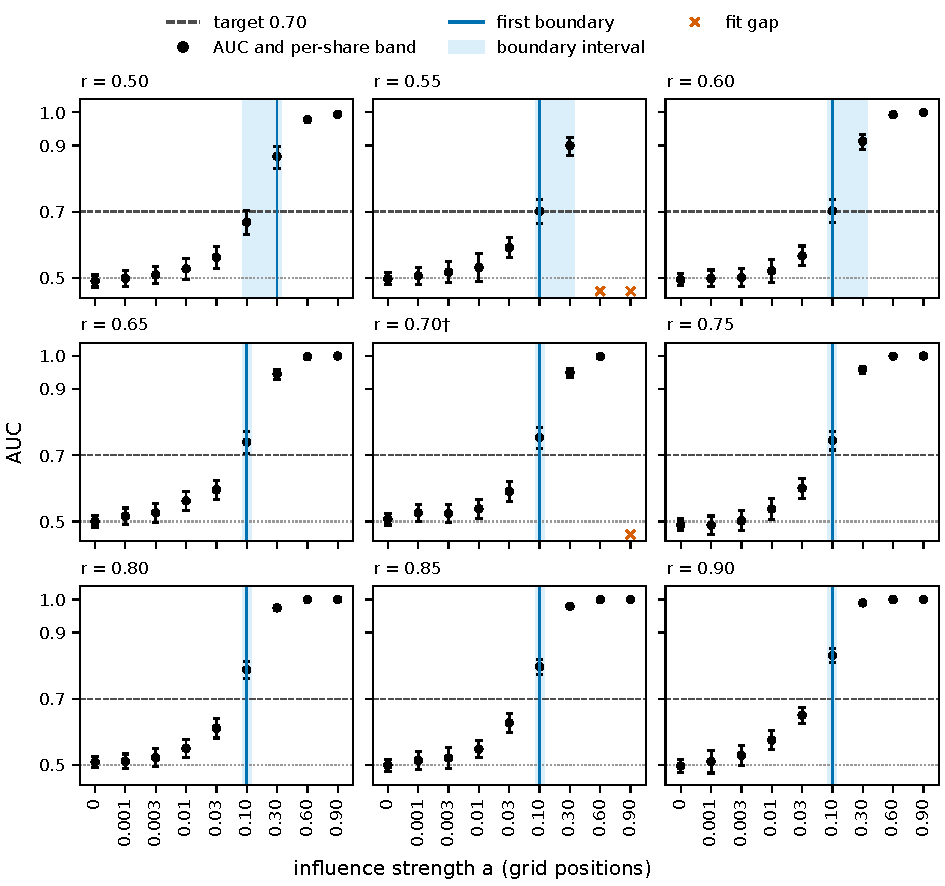
\includegraphics[width=\textwidth]{generated/J2_auc_profiles_B.pdf}
\caption{AUC profiles against trait-plus-autoregressive persistence (B), one panel per signal share $r$. Points are point AUCs; vertical bars show that share's band, simultaneous over strengths; the vertical line marks the first boundary and the shading its interval; crosses mark fit gaps. Dashed line: target \resultnum{j.target.r070}{0.70}. Dotted line: chance (\resultnum{j.chance}{0.5}). $\dag$ Examined during calibration.}\label{fig:auc-B}
\end{figure*}


\begin{table*}[tp]
\caption{Boundaries against trait-plus-autoregressive persistence (B).}\label{tab:boundaries-B}
\centering\scriptsize
\setlength{\tabcolsep}{5pt}
\begin{tabular}{l>{\raggedright\arraybackslash}p{22mm}>{\raggedright\arraybackslash}p{28mm}rrrrr}
\toprule
$r$ & $a^*$ [interval] & $a_s^*$ [interval] & \shortstack{AUC at\\\resultnum{j.grid.a0300}{0.03}} & \shortstack{AUC at\\\resultnum{j.grid.a1000}{0.10}} & \shortstack{AUC at\\\resultnum{j.grid.a3000}{0.30}} & \shortstack{Target\\\resultnum{j.target.r060}{0.60}} & \shortstack{Target\\\resultnum{j.target.r080}{0.80}} \\
\midrule
\resultnum{v4.tab.T1.B.r050.r}{0.50} & \resultnum{j.b.r050.first.point}{0.30} [\resultnum{j.b.r050.first.lower}{0.10}, \resultnum{j.b.r050.first.upper}{0.30}] & \resultnum{j.b.r050.sustained.point}{0.30} [\resultnum{j.b.r050.sustained.lower}{0.10}, \resultnum{j.b.r050.sustained.upper}{0.30}] & \resultnum{j.b.r050.a0300.auc}{0.562} & \resultnum{j.b.r050.a1000.auc}{0.668} & \resultnum{j.b.r050.a3000.auc}{0.867} & \resultnum{j.b.r050.target060.point}{0.10} & \resultnum{j.b.r050.target080.point}{0.30} \\
\resultnum{v4.tab.T1.B.r055.r}{0.55} & \resultnum{j.b.r055.first.point}{0.10} [\resultnum{j.b.r055.first.lower}{0.10}, \resultnum{j.b.r055.first.upper}{0.30}] & censored (fit gaps at \resultnum{j.b.r055.sustained.gap.0.a}{0.60}, \resultnum{j.b.r055.sustained.gap.1.a}{0.90}) & \resultnum{j.b.r055.a0300.auc}{0.591} & \resultnum{j.b.r055.a1000.auc}{0.702} & \resultnum{j.b.r055.a3000.auc}{0.900} & \resultnum{j.b.r055.target060.point}{0.10} & \resultnum{j.b.r055.target080.point}{0.30} \\
\resultnum{v4.tab.T1.B.r060.r}{0.60} & \resultnum{j.b.r060.first.point}{0.10} [\resultnum{j.b.r060.first.lower}{0.10}, \resultnum{j.b.r060.first.upper}{0.30}] & \resultnum{j.b.r060.sustained.point}{0.10} [\resultnum{j.b.r060.sustained.lower}{0.10}, \resultnum{j.b.r060.sustained.upper}{0.30}] & \resultnum{j.b.r060.a0300.auc}{0.567} & \resultnum{j.b.r060.a1000.auc}{0.702} & \resultnum{j.b.r060.a3000.auc}{0.913} & \resultnum{j.b.r060.target060.point}{0.10} & \resultnum{j.b.r060.target080.point}{0.30} \\
\resultnum{v4.tab.T1.B.r065.r}{0.65} & \resultnum{j.b.r065.first.point}{0.10} [\resultnum{j.b.r065.first.lower}{0.10}, \resultnum{j.b.r065.first.upper}{0.10}] & \resultnum{j.b.r065.sustained.point}{0.10} [\resultnum{j.b.r065.sustained.lower}{0.10}, \resultnum{j.b.r065.sustained.upper}{0.10}] & \resultnum{j.b.r065.a0300.auc}{0.596} & \resultnum{j.b.r065.a1000.auc}{0.740} & \resultnum{j.b.r065.a3000.auc}{0.946} & \resultnum{j.b.r065.target060.point}{0.10} & \resultnum{j.b.r065.target080.point}{0.30} \\
\resultnum{v4.tab.T1.B.r070.r}{0.70}\dag{} & \resultnum{j.b.r070.first.point}{0.10} [\resultnum{j.b.r070.first.lower}{0.10}, \resultnum{j.b.r070.first.upper}{0.10}] & censored (fit gap at \resultnum{j.b.r070.sustained.gap.0.a}{0.90}) & \resultnum{j.b.r070.a0300.auc}{0.591} & \resultnum{j.b.r070.a1000.auc}{0.754} & \resultnum{j.b.r070.a3000.auc}{0.950} & \resultnum{j.b.r070.target060.point}{0.10} & \resultnum{j.b.r070.target080.point}{0.30} \\
\resultnum{v4.tab.T1.B.r075.r}{0.75} & \resultnum{j.b.r075.first.point}{0.10} [\resultnum{j.b.r075.first.lower}{0.10}, \resultnum{j.b.r075.first.upper}{0.10}] & \resultnum{j.b.r075.sustained.point}{0.10} [\resultnum{j.b.r075.sustained.lower}{0.10}, \resultnum{j.b.r075.sustained.upper}{0.10}] & \resultnum{j.b.r075.a0300.auc}{0.600} & \resultnum{j.b.r075.a1000.auc}{0.745} & \resultnum{j.b.r075.a3000.auc}{0.959} & \resultnum{v4.tab.T1sec.B.r075.a060.1}{0.03} & \resultnum{j.b.r075.target080.point}{0.30} \\
\resultnum{v4.tab.T1.B.r080.r}{0.80} & \resultnum{j.b.r080.first.point}{0.10} [\resultnum{j.b.r080.first.lower}{0.10}, \resultnum{j.b.r080.first.upper}{0.10}] & \resultnum{j.b.r080.sustained.point}{0.10} [\resultnum{j.b.r080.sustained.lower}{0.10}, \resultnum{j.b.r080.sustained.upper}{0.10}] & \resultnum{j.b.r080.a0300.auc}{0.611} & \resultnum{j.b.r080.a1000.auc}{0.788} & \resultnum{j.b.r080.a3000.auc}{0.975} & \resultnum{v4.tab.T1sec.B.r080.a060.1}{0.03} & \resultnum{j.b.r080.target080.point}{0.30} \\
\resultnum{v4.tab.T1.B.r085.r}{0.85} & \resultnum{j.b.r085.first.point}{0.10} [\resultnum{j.b.r085.first.lower}{0.10}, \resultnum{j.b.r085.first.upper}{0.10}] & \resultnum{j.b.r085.sustained.point}{0.10} [\resultnum{j.b.r085.sustained.lower}{0.10}, \resultnum{j.b.r085.sustained.upper}{0.10}] & \resultnum{j.b.r085.a0300.auc}{0.627} & \resultnum{j.b.r085.a1000.auc}{0.797} & \resultnum{j.b.r085.a3000.auc}{0.979} & \resultnum{v4.tab.T1sec.B.r085.a060.1}{0.03} & \resultnum{j.b.r085.target080.point}{0.30} \\
\resultnum{v4.tab.T1.B.r090.r}{0.90} & \resultnum{j.b.r090.first.point}{0.10} [\resultnum{j.b.r090.first.lower}{0.10}, \resultnum{j.b.r090.first.upper}{0.10}] & \resultnum{j.b.r090.sustained.point}{0.10} [\resultnum{j.b.r090.sustained.lower}{0.10}, \resultnum{j.b.r090.sustained.upper}{0.10}] & \resultnum{j.b.r090.a0300.auc}{0.650} & \resultnum{j.b.r090.a1000.auc}{0.831} & \resultnum{j.b.r090.a3000.auc}{0.990} & \resultnum{v4.tab.T1sec.B.r090.a060.1}{0.03} & \resultnum{j.b.r090.target080.point}{0.10} \\
\botrule
\end{tabular}
\par\smallskip\parbox{\linewidth}{$r$ is signal share in the continuous response before discretization. $a^*$: first boundary [interval from the band]; $a_s^*$: sustained boundary; censored: not declared across fit gaps. All \resultnum{j.b.first.large.n}{9} first-boundary intervals lie entirely above \resultnum{j.grid.a0300}{0.03}. AUC columns give point estimates; target columns give first boundaries at secondary targets. \dag{} Examined during calibration. Definitions: \esmresource, Table~\ref{esm-tab:glossary-terms}.}
\end{table*}


Two descriptive readings qualify this curve. The flat boundary hides a dependence on $r$ that the coarse grid absorbs: the AUC at $a=0.10$ ranged from \resultnum{j.b.a1000.auc.min}{0.668} at $r=\resultnum{j.b.a1000.auc.min.r}{0.50}$ to \resultnum{j.b.a1000.auc.max}{0.831} at $r=\resultnum{j.b.a1000.auc.max.r}{0.90}$, tending to rise with $r$, and at $r=0.55$ and $0.60$ it was \resultnum{j.b.r055.a1000.auc}{0.702} and \resultnum{j.b.r060.a1000.auc}{0.702}, close to the target, so the intervals there extend to $a=\resultnum{j.b.r055.first.upper}{0.30}$. The arms already differed at $a=0.03$, where every lower band exceeded $0.5$ (the lowest was \resultnum{j.b.r050.a0300.lower}{0.528}, at $r=0.50$) and every upper band stayed below $0.70$ (the highest was \resultnum{j.b.a0300.upper.max}{0.675}, at $r=\resultnum{j.b.a0300.upper.max.r}{0.90}$). The boundary therefore marks a performance target, not the first detectable difference; the conjunction of nine intervals above $0.03$ carries no joint error rate. These readings were made after the results became available. Point AUCs, band limits and critical values for all \resultnum{v4.protocol.grid_cells}{81} cells are in \esmresource, Tables~\ref{esm-tab:b-cells}--\ref{esm-tab:b-cells-part-c}.

\subsection{Eligibility of the other persistence comparisons}\label{sec:results-other}

Table~\ref{tab:other-models} summarizes the secondary persistence models, whose AUC profiles are in \esmresource, Figs.~\ref{esm-fig:auc-A}--\ref{esm-fig:auc-E}. Against autoregressive persistence (A) and mover--stayer persistence (E), all units were complete and valid, every first boundary was \resultnum{j.models.A.r055.first.point}{0.10} or \resultnum{j.models.A.r050.first.point}{0.30} with an interval above $0.03$, and every sustained boundary equaled the first or was censored by fit gaps at the top of the grid.

\begin{table*}[tp]
\caption{Boundaries against the other persistence models.}\label{tab:other-models}
\centering\scriptsize
\setlength{\tabcolsep}{4pt}
\begin{tabular}{ll>{\raggedright\arraybackslash}p{62mm}>{\raggedright\arraybackslash}p{54mm}}
\toprule
Model & $r$ & First boundary & Sustained boundary \\
\midrule
A & \resultnum{j.models.r050.r}{0.50} & \resultnum{j.models.A.r050.first.point}{0.30} & \resultnum{j.models.A.r050.sustained.point}{0.30} \\
A & \resultnum{j.models.r055.r}{0.55}--\resultnum{j.models.r090.r}{0.90} & \resultnum{j.models.A.r055.first.point}{0.10} & \resultnum{j.models.A.r055.sustained.point}{0.10} \\
C & All shares & Invalid: zero-strength AUC \resultnum{j.models.C.zero_auc.min}{1.000} & Suppressed \\
D & All shares & Censored at first gap: \resultnum{j.models.D.r055.first.censoring_gap.a}{0.10} at \resultnum{j.models.D.first_gap.a1000.family_limit.n}{7} shares (family limit on profile); \resultnum{j.models.D.r050.first.censoring_gap.a}{0.01} at $r=$ \resultnum{j.models.D.r050.r}{0.50} (other solver status); \resultnum{j.models.D.r060.first.censoring_gap.a}{0.003} at $r=$ \resultnum{j.models.D.r060.r}{0.60} (propagation gap) & Censored (fit gaps) \\
E & \resultnum{j.models.r050.r}{0.50}--\resultnum{j.models.r060.r}{0.60} & \resultnum{j.models.E.r050.first.point}{0.30} & \resultnum{j.models.E.r050.sustained.point}{0.30}; censored at $r=$ \resultnum{j.models.r055.r}{0.55} (fit gaps at \resultnum{j.models.E.r055.sustained.gap.0.a}{0.60}, \resultnum{j.models.E.r055.sustained.gap.1.a}{0.90}) \\
E & \resultnum{j.models.r065.r}{0.65}--\resultnum{j.models.r090.r}{0.90} & \resultnum{j.models.E.r065.first.point}{0.10} & \resultnum{j.models.E.r065.sustained.point}{0.10}; censored at $r=$ \resultnum{j.models.r070.r}{0.70} (fit gap at \resultnum{j.models.E.r070.sustained.gap.0.a}{0.90}) \\
\botrule
\end{tabular}
\par\smallskip\parbox{\linewidth}{$r$ is signal share in the continuous response before discretization. A: autoregressive; C: autoregressive with an altered response channel; D: state-dependent; E: mover--stayer. A and E group consecutive shares with the same first boundary; sustained-boundary exceptions are explicit. Unmarked entries are complete and valid; C is complete but invalid, so its boundaries are suppressed. Boundary and censoring definitions: \esmresource, Table~\ref{esm-tab:glossary-terms}; fit statuses: Table~\ref{esm-tab:glossary-states}.}
\end{table*}


All nine units of autoregressive persistence with an altered response channel (C) were complete but invalid. C has no zero-strength identity: it alters the response channel of the persistence arm only. The classifier separated the arms perfectly at zero strength, with a point AUC of \resultnum{j.models.C.zero_auc.min}{1.000} at every share. This failed the prespecified zero-strength eligibility check and suppressed C's boundaries. The failure reflects the channel asymmetry, not evidence about persistence or influence, and by itself establishes no implementation defect. Because the prespecified comparison across persistence models required every secondary unit to be complete and valid, that comparison was unavailable and its prespecified display of offsets between models was not produced. The valid units remain displayed without promoting or demoting a persistence model.

All nine units of state-dependent persistence (D) were complete and valid, but fit gaps censor every first and sustained boundary, beginning at seven shares at $a=0.10$, where B's boundary lies (Table~\ref{tab:other-models}). Of D's \resultnum{j.models.D.gaps.total}{38} gap cells, \resultnum{j.models.D.gaps.family_limit}{33}, including every gap at $a=0.10$, are family limits: the prespecified profile solver reached the edge of D's parameter box without an accepted match. It found no admissible match at $a=0.10$ or $0.30$, the strengths of B's first boundaries, at any share. These are limits of the declared matching procedure, not AUCs below the target or proof that no parameter in the box could match the moments (\esmresource, Section~\ref{esm-sec:additional-models}).

\subsection{Measurement controls and sensitivities}\label{sec:results-controls}

The measurement controls repeat the comparison on error-free responses, reusing the second persistence parameter of the observed fit (\esmresource, Table~\ref{esm-tab:controls}). Against B, the ordinal control, discretized without error ($r=1$), and the latent-rank control reached the target at $a=\resultnum{j.controls.ordinal_one.r050.first.point}{0.10}$ at every share; only the latent control, with neither error nor discretization, reached it at $a=\resultnum{j.controls.latent.r055.first.point}{0.03}$, at \resultnum{j.controls.latent.n_boundary_a0300}{8} shares. Removing response error while retaining ordinal allocation left the point boundary unchanged at design shares from $r=0.55$ to $0.90$, but at $r=0.50$ it fell from $a=\resultnum{j.b.r050.first.point}{0.30}$ to $a=\resultnum{j.controls.ordinal_one.r050.first.point}{0.10}$.

Of the \resultnum{j.sensitivity.n_pairs_compared}{63} complete and valid sensitivity units, \resultnum{j.sensitivity.n_region_differs}{8} differed from the main curve in whether the first boundary was declared with an interval entirely above $a=0.03$ (\esmresource, Section~\ref{esm-sec:additional-controls}). Without repulsion ($b=0$), the first boundary was \resultnum{j.sensitivity.b000.first.min}{0.03} to \resultnum{j.sensitivity.b000.first.max}{0.10} at every share, with intervals reaching down to \resultnum{j.sensitivity.b000.r080.sensitivity.lower}{0.03} at $r=0.80$ to $0.90$, so repulsion is not needed for detection; with persistent response style or panel conditioning in both arms, \resultnum{j.sensitivity.response_channel.n_same_region}{44} of \resultnum{v4.inv.t4.n_valid}{45} units kept the interval above $a=0.03$. With \resultnum{v4.protocol.steps}{24} updates per wave and the same per-step persistence, the annual process itself changes, as annual latent persistence without influence falls to $0.85^{24}$, close to zero; anchoring to the initial state, which B lacks, separated the arms without influence (zero-strength AUC \resultnum{j.sensitivity.omega025.zero_auc.min}{0.647} to \resultnum{j.sensitivity.omega025.zero_auc.max}{0.892} at the weakest anchoring) or could not be fitted, so it is uninformative about influence.

\subsection{Exploratory explanations of separation and fragility}\label{sec:results-exploratory}

Table~\ref{tab:exploratory} describes each exploratory analysis. All lie outside the confirmatory estimand; they examine the scale, sources and sensitivity of separation rather than independently confirming the main curve. The twin, variance and stress-test analyses were read when they finished and the others after the results became available; every comparison with the main curve is a later reading.

\begin{table*}[tp]
\caption{Exploratory analyses at a glance. All were declared before any confirmatory result, use seeds disjoint from the confirmatory ones and lie outside the confirmatory estimand. Ranges are minima and maxima over signal shares; the last column is a reading made after the results became available. Full results and definitions: Online Resource~1, Section~\ref{esm-sec:exploratory} and Table~\ref{esm-tab:glossary-terms}.}\label{tab:exploratory}
\centering\scriptsize
\setlength{\tabcolsep}{2.5pt}
\begin{tabular}{@{}p{0.10\textwidth}p{0.13\textwidth}p{0.285\textwidth}p{0.265\textwidth}p{0.17\textwidth}@{}}
\toprule
\raggedright Analysis & \raggedright Question & \raggedright What changes relative to the main design & \raggedright Main result & \raggedright Reading \tabularnewline
\midrule
\raggedright Mean-field twin & \raggedright Is the persistent input from fixed contacts needed? & \raggedright Influence term replaced by fresh Gaussian noise with its mean and variance given the own state: keeps the own-state effect, removes the persistent input, the dependence between people and the term's shape & \raggedright Arm against twin at $a=0.10$: AUC \resultnum{j.x1a.auc.a010.min}{0.623}--\resultnum{j.x1a.auc.a010.max}{0.716}; mean lag correlations differing by at most \resultnum{j.x1a.lag_difference.a010.max}{0.0056}, positive at every lag and growing with it. Twin against B: target reached only at $r=0.90$, at $a=\resultnum{j.x1b.r090.first.point}{0.30}$ & \raggedright Separation does not come from the own-state effect alone; not network-specific; may include the start-up transient \tabularnewline
\raggedright Variance explained by influence & \raggedright What does a nominal strength mean on a variance scale? & \raggedright Latent paths without response channel; partial $R^2$ of the standardized influence term for the next latent attitude beyond linear persistence & \raggedright Partial $R^2$ \resultnum{j.x2a.a003}{0.016}, \resultnum{j.x2a.a010}{0.054} and \resultnum{j.x2a.a030}{0.167} at $a=0.03$, $0.10$ and $0.30$; a natural cubic spline of the own state with five knots absorbed little of it & \raggedright Little latent variance at the boundary; per-step latent scale; spline result specific to that spline \tabularnewline
\raggedright Free signal share & \raggedright Does separation survive when B fits its signal share? & \raggedright B fits its signal share with its two parameters to lags 1--3; both contrasts classify on lags 4--5 only & \raggedright At the first boundary, AUC \resultnum{j.x3.known.auc.min}{0.668}--\resultnum{j.x3.known.auc.max}{0.858} with the share known and \resultnum{j.x3.free.auc.min}{0.534}--\resultnum{j.x3.free.auc.max}{0.585} with it free; fitted share \resultnum{j.x3.free.r_shift.min}{0.0011}--\resultnum{j.x3.free.r_shift.max}{0.0028} below the true one; free-share interval below $0.70$ where the known-share AUC reached it in \resultnum{j.x3.lost_crossings.n}{18} of \resultnum{j.x3.lost_crossings.cells}{21} cells at $a=0.10$--$0.60$ & \raggedright One fit, contributions not disentangled, absorbed most separation; sensitive to reliability in the third decimal; matching uncertainty omitted \tabularnewline
\raggedright Oracle single-panel test & \raggedright How often does one panel reject B? & \raggedright New influence panels scored against \resultnum{v4x.x4.sizes.check_prose}{4,000} null scores of the fitted B; discriminant direction trained on the true alternative & \raggedright Rejection at the first boundary \resultnum{j.x4a.boundary_rejection.min}{0.171}--\resultnum{j.x4a.boundary_rejection.max}{0.368} at $r\ge0.55$ and \resultnum{j.x4a.boundary_rejection.r050}{0.447} at $r=0.50$ & \raggedright A reference with privileged information, of the size Table~\ref{tab:auc-translation} suggests \tabularnewline
\raggedright Fitted single-panel test & \raggedright Can B be fitted to one panel and tested by bootstrap? & \raggedright B fitted to one panel's lags 1--2; the panel's score compared with \resultnum{v4x.x4.sizes.nulls}{199} null panels simulated at the fit; the same trained direction & \raggedright Rejection \resultnum{j.x4b.zero_rejection.r050}{0.300} at $a=0$, $r=0.50$, and \resultnum{v4x.x4.x4b.r070.a0010.x4b.power_pu}{0.33} at $a=0.001$, $r=0.70$, nominal level \resultnum{v4x.protocol.x4.level}{0.05} & \raggedright Not a valid procedure; discrepancy with the oracle test unexplained \tabularnewline
\raggedright Channel-\hspace{0pt}mis\-spec\-i\-fi\-ca\-tion stress test & \raggedright How much separation does a misspecified channel alone produce? & \raggedright $a=0$; influence arm observed through a misspecified channel (signal-share trend across waves, step at wave five, panel conditioning, trust-dependent attrition, in the SHP's direction \cite{lipps2007,voorpostel2010}); B fitted with the assumed one & \raggedright Trend of $\pm0.03$: AUC \resultnum{j.x5.trend003.min}{0.680}--\resultnum{j.x5.trend003.max}{0.710}; $\pm$\resultnum{j.x5.trend.amplitude_large}{0.08}: \resultnum{j.x5.trend008.min}{0.884}--\resultnum{j.x5.trend008.max}{0.907}; attrition with retention odds ratio \resultnum{j.x5.attrition.odds_ratio_small}{1.5}: \resultnum{j.x5.attrition15.min}{0.540}--\resultnum{j.x5.attrition15.max}{0.640}, with 2: \resultnum{j.x5.attrition2.min}{0.578}--\resultnum{j.x5.attrition2.max}{0.820}; step and conditioning not fitted & \raggedright Misspecification alone reaches the target with influence's sign pattern (all \resultnum{j.x5.signature.cells}{36} estimated cells below B at lags 3--5, growing with the lag): detection is not attribution \tabularnewline
\raggedright Band coverage check & \raggedright Do the bands cover the procedural truth at positive strength? & \raggedright \resultnum{v4x.x6.x6a.band.vs_d1.gaps_as_misses.total}{200} repetitions of the whole unit at $r=0.70$; \resultnum{v4x.x6.x6b.cells.r050.a0300.vs_d1.pointwise.total}{200} pipelines at $a=0.03$ with $r=0.50$ and with $r=0.90$; procedural truth: expected AUC of the prespecified procedure & \raggedright \resultnum{v4x.x6.x6a.band.vs_d1.primary.covered}{162} of \resultnum{v4x.x6.x6a.band.vs_d1.primary.total}{166} complete gap-free bands covered (\resultnum{v4x.x6.x6a.band.vs_d1.primary.wilson95.prose_lower}{0.940}--\resultnum{v4x.x6.x6a.band.vs_d1.primary.wilson95.prose_upper}{0.991}); \resultnum{v4x.x6.x6a.band.vs_d1.gaps_as_misses.covered}{162} of \resultnum{v4x.x6.x6a.band.vs_d1.gaps_as_misses.total}{200} counting gaps as misses (\resultnum{j.x6.gaps_as_misses.wilson.lower}{0.750}--\resultnum{j.x6.gaps_as_misses.wilson.upper}{0.858}); pointwise \resultnum{v4x.x6.x6b.cells.r050.a0300.vs_d1.pointwise.covered}{193} and \resultnum{v4x.x6.x6b.cells.r090.a0300.vs_d1.pointwise.covered}{189} of \resultnum{v4x.x6.x6b.cells.r090.a0300.vs_d1.pointwise.total}{200} at $a=0.03$ & \raggedright No undercoverage detected for complete bands or at $a=0.03$; failure when gaps count as misses \tabularnewline
\raggedright Expanded-feature classifier & \raggedright How far does the boundary fall with more features? & \raggedright Thirty-six pooled features, none chosen by search: lag correlations at lags 3--10, one-wave change by tercile, lag-1 transitions between five category groups and quantiles of within-person SD. Same arms, fit and classifier code & \raggedright First boundary \resultnum{j.x7.first.min}{0.003}--\resultnum{j.x7.first.max}{0.03} at every share, against \resultnum{j.x7.frozen_first.min}{0.10}--\resultnum{j.x7.frozen_first.max}{0.30} with three features; largest AUC gain at $a=0.03$: \resultnum{j.x7.auc_gain.a0300.max}{0.339}; gain already at $a=0.001$, although paired intervals also excluded zero at $a=0$ at $r=0.65$ and $0.80$ & \raggedright Richer summaries separate these laws at lower strengths; specificity to influence not assessed \tabularnewline
\botrule
\end{tabular}
\end{table*}


\paragraph{Independent-seed reruns.} Two exploratory reruns of the frozen pipeline on independent seeds kept every first boundary above $a=0.03$ (the largest oracle reference AUC there was \resultnum{j.x4a.a0300.auc_ref.max}{0.638}), but the point boundary changed near the target: at $r=0.55$ one rerun gave $a=\resultnum{j.x7.frozen_first.r055}{0.30}$, and the other an AUC of \resultnum{j.x4a.r055.a1000.auc_ref}{0.683} at $a=0.10$ (interval \resultnum{j.x4a.r055.a1000.auc_ref.lower}{0.672}--\resultnum{j.x4a.r055.a1000.auc_ref.upper}{0.694}). These reruns show the sensitivity of a point boundary on a coarse grid near the chosen target.

\paragraph{Free signal share.} Here B fits its signal share and its two persistence parameters to the lag-one to lag-three correlations, and both contrasts classify on lags four and five only. Letting B fit its share while matching lag three as well lowered the lag-four-and-five AUC at the first boundary from \resultnum{j.x3.known.auc.min}{0.668}--\resultnum{j.x3.known.auc.max}{0.858} to \resultnum{j.x3.free.auc.min}{0.534}--\resultnum{j.x3.free.auc.max}{0.585} (\esmresource, Section~\ref{esm-sec:x3}). The fit did this by lowering the share by only \resultnum{j.x3.free.r_shift.min}{0.0011} to \resultnum{j.x3.free.r_shift.max}{0.0028}, which more than halved B's trait weight; at the true share, B missed the lag-three correlation by \resultnum{j.x3.l3_miss_se.abs.min}{7.1} to \resultnum{j.x3.l3_miss_se.abs.max}{13.4} standard errors of the matching fit. The share shift and the extra matched lag are one fit whose contributions were not disentangled, and the contrast omits the uncertainty of the three-parameter matching. In \resultnum{j.x3.lost_crossings.n}{18} of the \resultnum{j.x3.lost_crossings.cells}{21} cells at $a=0.10$ to $0.60$ where both contrasts were estimated, the known-share AUC reached $0.70$ while the free-share interval stayed below it, a count of successful cells rather than a corrected inference; no free-share point AUC reached $0.70$ wherever that fit succeeded.

\paragraph{Single-panel tests.} Both procedures score a panel along the discriminant direction trained on the true alternative, which an analyst would not have. At zero strength, the oracle test's rejection rate was compatible with the nominal \resultnum{v4x.protocol.x4.level}{0.05} except at $r=0.70$ (\resultnum{v4x.x4.x4a.r070.a0000.x4a.power_or}{0.069}). The fitted test is closer to an analyst's procedure but is not a valid one: without influence, at $r=0.50$, it rejected B in \resultnum{j.x4b.zero_rejection.r050}{0.300} of panels (interval \resultnum{j.x4b.zero_rejection.r050.lower}{0.235} to \resultnum{j.x4b.zero_rejection.r050.upper}{0.365}). Under very weak influence ($a=0.001$, $r=0.70$), the fitted test rejected \resultnum{v4x.x4.x4b.r070.a0010.x4b.power_pu}{0.33} of panels and the oracle test \resultnum{v4x.x4.x4a.r070.a0010.x4a.power_or}{0.051}, a discrepancy whose source was not isolated.

\paragraph{Channel-misspecification stress test.} Without influence, at $r=0.60$ to $0.90$, the AUC under the $\pm0.03$ trend lay between the confirmatory AUCs at $a=0.03$ and $0.10$, and every estimated interval excluded $0.5$.

\paragraph{Band coverage check.} At $r=0.70$, \resultnum{v4x.x6.x6a.band.vs_d1.primary.covered}{162} of the \resultnum{v4x.x6.x6a.band.vs_d1.primary.total}{166} complete, gap-free bands covered the procedural truth at all nine strengths, read under the prespecified criterion as no undercoverage detected; counting the \resultnum{v4x.x6.x6a.strengths.r070.a0000.gaps}{34} repetitions with a gap as misses gives \resultnum{v4x.x6.x6a.band.vs_d1.gaps_as_misses.covered}{162} of \resultnum{v4x.x6.x6a.band.vs_d1.gaps_as_misses.total}{200} (\resultnum{j.x6.gaps_as_misses.percent}{81}\%), a failure that mixes unavailable bands with noncoverage. At $a=0.03$ no undercoverage was detected.

\paragraph{Expanded-feature classifier.} The gain over three features was already positive at $a=0.001$ at every share, with paired intervals above zero, although at zero strength, where the two laws coincide, the paired intervals also excluded zero at $r=0.65$ and $0.80$. More features change estimation and regularization as well as information, so neither boundary marks the limit of what the panels contain.


\section{Discussion}\label{sec:discussion}
This Discussion interprets the results after they became available; the prespecified reading rules are archived with the code (\esmresource, Section~\ref{esm-sec:rule-record}). The central issue is how far discrimination between the simulated laws supports a claim about social influence. Three design limitations govern that interpretation: the restricted persistence alternatives, privileged knowledge of the response channel, and observation before the network process has had a burn-in.

\subsection{What classifier separation establishes}\label{sec:disc-meaning}

The confirmatory curve, $a^*(r)=\resultnum{j.b.r055.first.point}{0.10}$ for $r=0.55$--$0.90$ and \resultnum{j.b.r050.first.point}{0.30} at $r=0.50$, describes one classifier on three pooled long-lag correlations against trait-plus-autoregressive persistence. It holds with $r$ known, persistence matched to population moments, a correct response channel and panels as large as the SHP. AUC measures how well the classifier ranks panels drawn from these two simulated laws; the $0.70$ target is neither classification accuracy nor the power to reject persistence in one panel. Under the equal-variance normal approximation at a one-sided 5\% level, that target corresponds to single-panel power of about \resultnum{j.auc_translation.target070.power}{0.18} against a known persistence score distribution (Table~\ref{tab:auc-translation}). The curve therefore demonstrates conditional discrimination, without identifying social influence.

The parameter $a$ is a nominal innovation-variance fraction, not a realized share of attitude change or an empirical measure of social influence intensity. In the exploratory variance analysis, the influence term explains \resultnum{j.x2a.a010}{0.054} of the variance of the next latent attitude left after linear persistence at $a=0.10$, and \resultnum{j.x2a.a003}{0.016} at $a=0.03$. These are per-step latent quantities, not observed-scale effects. At the first-boundary cells, whose AUCs exceed $0.70$ on the coarse grid, even the oracle test rejected B for only \resultnum{j.x4a.boundary_rejection.min}{0.171} to \resultnum{j.x4a.boundary_rejection.max}{0.368} of single panels at $r\ge0.55$. It rejected B in at least four of five panels only from $a=0.30$ at $r\ge0.75$ (\resultnum{v4x.x4.x4a.r075.a3000.x4a.power_or}{0.826} to \resultnum{v4x.x4.x4a.r090.a3000.x4a.power_or}{0.944}), where influence explains \resultnum{j.x2a.a030}{0.167} of that residual variance; at $r=0.70$ and $a=0.30$ it rejected \resultnum{v4x.x4.x4a.r070.a3000.x4a.power_or}{0.759}. These exploratory rejection rates are references with privileged information, not the performance of an available empirical test.

The numerical boundary also depends on the target and the summaries. At the secondary target of \resultnum{v4.protocol.secondary_target.lower}{0.60} it falls to $a=\resultnum{v4.tab.T1sec.B.r075.a060.1}{0.03}$ at $r=0.75$ to $0.90$. In the exploratory comparison, thirty-six features reached the primary target at $a=\resultnum{j.x7.first.min}{0.003}$ to \resultnum{j.x7.first.max}{0.03} on the same panels on which three needed \resultnum{j.x7.frozen_first.min}{0.10} to \resultnum{j.x7.frozen_first.max}{0.30}. B was matched to none of the added features, and their gain changes estimation and regularization as well as information. Its source and specificity to influence were not isolated. The three-feature boundary is thus a property of the declared procedure, not a limit on all information in these panels.

\subsection{Restricted persistence alternatives}\label{sec:disc-mechanism}

The persistence alternatives do not span the temporal processes that could rival influence. Apart from transport and discretization, A, B and E share a plateau plus a single exponential decay, with no plateau for A. Their displayed boundaries cannot serve as independent corroboration, and the prespecified comparison across all persistence models was unavailable because C was invalid. D's boundaries were censored by matching gaps, so that comparison did not establish whether the classifier could distinguish influence from matched non-Gaussian state-dependent persistence.

The exploratory mean-field twin helps explain what this restricted family may miss. At $a=0.10$ the influence arm and its twin differed by at most \resultnum{j.x1a.lag_difference.a010.max}{0.0056} in mean lag correlation, yet the classifier separated them with AUCs of \resultnum{j.x1a.auc.a010.min}{0.623} to \resultnum{j.x1a.auc.a010.max}{0.716}. The twin keeps the effect through the own state while replacing the input from fixed contacts by fresh Gaussian noise. This contrast also changes dependence between people and the term's distribution, so it does not isolate a network-specific contribution. It is consistent with persistent contact input being an important source of separation, but does not establish that explanation (Section~\ref{sec:methods-identification}).

A persistent input can slow the decay of within-person correlations relative to a single exponential; B can mimic this with its plateau while missing the longer lags. In the free-share records, the influence arm's mean lag correlations at every boundary cell fell below those of known-share B at lags three to five, increasingly with the lag (at $r=0.70$, $\resultnum{j.x3.lag_shortfall.r070.l3}{-0.0011}$, $\resultnum{j.x3.lag_shortfall.r070.l4}{-0.0035}$ and $\resultnum{j.x3.lag_shortfall.r070.l5}{-0.0070}$). This is an observed lag pattern in the exploratory panels, not a decomposition of its causes.

No rival with serially correlated innovations, a second-order autoregression, or a sum of fast and slow autoregressive components was tested \cite{granger1976,asparouhov2018}. Nor did the design evaluate person-specific trends or persistence speeds \cite{bollencurran2004,asparouhov2018}, changes over the life course \cite{alwinkrosnick1991,lersch2023}, or period shocks shared by groups, which are relevant to trust in government. Such processes could reproduce part of the long-lag pattern and raise the boundary, possibly beyond the grid, but that possibility was not evaluated. Neither the mean-field twin nor the free-share analysis demonstrates what a matched second-order or two-component autoregressive rival would do. Testing those rivals, with heterogeneous persistence and matching at lags one to three, is needed before interpreting B's boundary as robust to richer individual dynamics.

\subsection{Privileged knowledge of response reliability}\label{sec:disc-attribution}

The confirmatory comparison gives both laws the same known signal share. With one answer per wave, estimating that share requires assumptions about the latent dynamics, so the restriction helps separate the laws through the very lag structure at issue (Section~\ref{sec:methods-identification}). A correctly specified channel shared by both arms changed little: \resultnum{j.sensitivity.response_channel.n_same_region}{44} of \resultnum{v4.inv.t4.n_valid}{45} sensitivity units kept the boundary interval above $a=0.03$. The exploratory analyses nevertheless show that allowing persistence to fit the channel, or misspecifying it, materially changes separation.

When B fitted its signal share to match lag three as well, most separation on lags four and five disappeared. The share moved by only \resultnum{j.x3.free.r_shift.min}{0.0011} to \resultnum{j.x3.free.r_shift.max}{0.0028} below the true value, more than halving B's trait weight. In the other direction, raising the share by \resultnum{j.x3.plus.offset}{0.01} moved that weight from \resultnum{j.x3.known.lambda.min}{0.139}--\resultnum{j.x3.known.lambda.max}{0.363} to \resultnum{j.x3.plus.lambda.min}{0.376}--\resultnum{j.x3.plus.lambda.max}{0.596}, with lags one and two matched in both cases. No free-share point AUC reached $0.70$ wherever that fit succeeded, although at $a=0.30$ and $r=0.90$ its interval reached $0.70$; in the four successful cells at $a=0.60$, the fit reduced B to an autoregression without trait. The share shift and extra matched lag are one fit whose contributions were not disentangled, and matching uncertainty was omitted. This is a demonstrated sensitivity of the lag-four-and-five classifier, not a revised confirmatory boundary or proof that the full laws are indistinguishable.

For the continuous response, a slightly lower share is equivalent to the true share with a short-lived latent component of corresponding size. Quasi-simplex models count such a component as error \cite{saris2014}, so this fit cannot tell slightly misjudged reliability from additional short-lived true variation. A share set \resultnum{j.x3.plus.offset}{0.01} too high put B's lag-three correlation \resultnum{j.x3.plus.l3_miss.min}{0.0069} to \resultnum{j.x3.plus.l3_miss.max}{0.0081} above the influence panels' at the boundary cells, the sign observed under influence. The response channel can also create separation when influence is absent: a misspecified channel reached AUCs up to \resultnum{j.x5.trend008.max}{0.907} (Table~\ref{tab:exploratory}). Unreliable items can make stable attitudes look changeable \cite{achen1975,ansolabehere2008}; a misspecified channel can also make persistence depart from the assumed model in influence's direction.

In that stress test, the arm without influence fell below B at lags three to five in all \resultnum{j.x5.signature.cells}{36} estimated cells, with a shortfall growing with the lag. Its median lag-five to lag-three ratio was \resultnum{j.x5.signature.ratio_l5_l3.median.mnar-ln15}{4.0} to \resultnum{j.x5.signature.ratio_l5_l3.median.trend-008}{4.8} by condition, against \resultnum{j.x3.lag_shortfall.ratio_l5_l3.min}{5.8} to \resultnum{j.x3.lag_shortfall.ratio_l5_l3.max}{6.9} under influence; individual cells overlap (\esmresource, Table~\ref{esm-tab:x5-lags}). Whether these departures would fool a score trained on influence was not evaluated. Neither the stress test nor the free-share contrast was run with the thirty-six features. They explain fragility within their declared comparisons, without establishing that every classifier would have the same sensitivity.

The SHP trust item illustrates the difficulty of supplying the privileged information (\esmresource, Section~\ref{esm-sec:shp}). An eleven-wave quasi-simplex model estimates reliability in \resultnum{v4.protocol.shp.anchor_year}{2004} at \resultnum{v4.shp.estimate}{0.674} and a trait--state--error fit at \resultnum{j.shp.starts.estimate}{0.696}, but the quasi-simplex fit is strained (persistence \resultnum{j.shp.multiwave.persistence}{0.961}; residual correlations up to \resultnum{j.shp.multiwave.max_cc_residual}{0.078}). Both models count stable response style as signal, whereas the simulation treats it as error: they estimate reliability, while the simulated signal share is closer to measurement quality \cite{saris2014}. If the latent process is a first-order autoregression with independent errors, Heise's coefficient \cite{heise1969} estimates a three-wave window's middle-wave reliability. Eight of the nine windows of \resultnum{j.shp.heise.w1999.start}{1999}--\resultnum{j.shp.heise.w2007.end}{2009} lie within \resultnum{j.shp.heise.others.spread}{0.029} of each other (standard errors \resultnum{j.shp.heise.w2004.se}{0.011} to \resultnum{j.shp.heise.w2002.se}{0.014}). The window of \resultnum{j.shp.heise.w2003.start}{2003}--\resultnum{j.shp.heise.w2003.end}{2005}, centered on refreshment-sample entry, lies \resultnum{j.shp.heise.dip2003}{0.065} below its neighbors' mean, giving a spread of \resultnum{j.shp.heise.spread}{0.077} including it. Sampling error, composition and departures from the model may all contribute; the spread does not estimate drift.

These standard errors provide a comparison of scales with the simulation's third-decimal sensitivity, not an empirical reliability threshold. A trend from $r-0.03$ to $r+0.03$ already separated simulated panels without influence. The short-lived response component, including error and short-lived true variation, is identified from one answer per wave only through the lag structure the classifier reads; assessing it at that precision would require several indicators or repeated measurement within a wave. Under this generator and channel, shares near the item's estimates gave $a=\resultnum{j.b.r065.first.point}{0.10}$ against B. This is not an estimated threshold for the SHP item: its lag profile, heaping at 0, 5 and 10, and attrition were never compared with the synthetic panels. An empirical analyst must also estimate persistence from one panel, rather than population moments. No valid analyst-implementable single-panel procedure was evaluated, so the curve does not establish the power available in that setting.

\subsection{Observation without network burn-in}\label{sec:disc-initialization}

The influence process begins from states unrelated to the network. With per-wave persistence of 0.85 and contacts fixed from wave 0, dependence between a person and those contacts plausibly takes several waves to build. The observed waves include that adjustment, which could contribute to the lag pattern used for discrimination. No analysis compared these panels with panels observed after burn-in. The contribution of the transient, and the direction in which burn-in would move the boundary, are therefore unknown. The mean-field contrast does not isolate this contribution either.

Other generator assumptions also limit transfer to empirical panels: one persistence and repulsion setting, eight contacts drawn uniformly at random and fixed for eleven years, perfect perception of their states, one step per wave, no coupling within households, and attrition that is neither selective nor temporary. The influence arm has no stable trait, whereas the SHP anchor's trait--state--error fit puts \resultnum{j.shp.starts.trait_share_2004}{0.758} of latent variance in a trait (\esmresource, Section~\ref{esm-sec:shp-results}). Influence confined to a smaller state component could require stronger input; fewer contacts could enlarge the persistent input and lower the boundary; homophily \cite{mcpherson2001}, clustering, contact turnover and noisy perception could fold it into own persistence or fresh noise and raise the boundary. These are untested mechanism-based conjectures, not sensitivity results. Adding a stable trait and comparing initialization with and without burn-in would address distinct parts of this scope.

\subsection{Relation to earlier work}\label{sec:disc-literature}

The ambiguity that Kiley and Vaisey describe between frequent updating and settled dispositions measured with error \cite{kiley2020} also arises between network influence and persistence, and turns on the response channel. Comparisons with no-change baselines \cite{moor2026,coding2024} do not match persistence to the same short-term stability; the boundary is a trajectory-level counterpart of the minimum change that Moor-Smith and Carpentras find a generator needs to beat no change. The stress test is a dynamic counterpart of measurement distortions in opinion-dynamics models \cite{carpentras2022,carpentras2023} and of spurious cross-lagged effects without a stable trait \cite{lucas2023}.

The result also raises a question about calibrations such as Gestefeld and Lorenz's to the same SHP item, in which each agent interacts with a randomly selected agent, or returns to its initial opinion, about 24 times per survey year \cite{gestefeld2023}. No persistent input from the same contacts builds up. At their best fits' return probability of 0.1 per step, about nine in ten agents return between annual waves, so year-to-year dependence runs largely through the initial opinion, a stable trait in panel terms. The closest analog here is the mean-field twin, which redraws the contact input at every step; against B it reached the target only at $r=0.90$, at $a=\resultnum{j.x1b.r090.first.point}{0.30}$. Neither the Gaussian twin nor the 24-step or anchoring sensitivity represents their model. If persistent input carries much of the present separation, random encounters could leave less separable panel transitions; this is a hypothesis for those calibrations, not a result about them. Their transition fit alone does not show that interaction is needed without comparison with matched persistence passed through the same response channel (Section~\ref{sec:implications}).

Without exposure data or other identifying restrictions, panels like these can establish a departure only from the persistence models considered. This meets the older problem of distinguishing contagion or state dependence from heterogeneity \cite{feller1943,heckman1981,gelastopoulos2025}; even with observed networks, separating influence from correlated effects and homophily requires strong assumptions \cite{manski1993,shalizi2011}.

\subsection{Further scope, uncertainty and reproducibility limits}\label{sec:limitations}

With 10,626 people and eleven waves, pooled correlations are very precise. Fewer people or waves would be expected to reduce that precision, and three-wave panels have no lags three to five. The grid starts at $r=0.50$, while many single items are less reliable \cite{hout2016,ansolabehere2008}. The channel is classical error around a latent state, discretized by within-wave ranks; answers that sample momentary considerations \cite{zaller1992} were not modeled, and the attrition result depends on pooling all available pairs of answers.

Inference at positive strength rests on limited checks. Band coverage was checked over the grid only at $r=0.70$, and pointwise at $a=0.03$ with $r=0.50$ and $0.90$. No undercoverage was detected for complete gap-free bands or at those pointwise cells; counting gaps as misses failed the coverage criterion (Section~\ref{sec:results-exploratory}). Near $a=0.03$, two gate diagnostics point in opposite directions (\esmresource, Section~\ref{esm-sec:record-gate}). With point estimates and critical values held fixed, an upper band at $a=0.03$ would reach $0.70$ only with a standard error about \resultnum{j.b.margin.a0300.se_factor.min}{2.0} times larger (at $r=\resultnum{j.b.margin.a0300.se_factor.min.r}{0.90}$; more elsewhere), whereas the nuisance-variance check at $r=0.70$ implies growth of at most about \resultnum{j.gate.g2c.a0300.se_growth_max}{1.46} times, and its applicability at other shares was not assessed. The zero-width interval at $r=0.65$ could widen by one grid step within the dispersion observed at $a=0.10$ and $r=0.70$.

The evaluation was not blind: at $r=0.70$ an earlier calibration proposal had shown an AUC of \resultnum{j.exposure.proposal_a.a010.mean}{0.756} at $a=0.10$ and \resultnum{j.exposure.proposal_a.a003}{0.589} at $a=0.03$, anticipating the boundary at that share. The AUC target and $0.03$ cut preceded these probes but not all earlier calibration (\esmresource, Section~\ref{esm-sec:record-exposure}). New seeds limit adaptation without removing it; the new confirmatory content is mainly the curve at the other eight shares.

Execution is bound to one recorded computing environment. Components agreed with independent implementations, but replay of the full pipeline has not been independently demonstrated, three frozen tests fail on Linux, and after an operating-system update on 9 October, that machine itself no longer passes the freeze check. The library entry points provide a route to rerun the simulation outside that environment, with possible floating-point and tolerance-edge differences. Agreement of such a complete rerun with the released results remains to be assessed (Data and code availability; \esmresource, Section~\ref{esm-sec:verification}).

\subsection{Implications for empirical work}\label{sec:implications}

For calibrating opinion-dynamics models to panel surveys, the findings support comparing influence with persistence matched to the same short-term stability, judging fit on patterns not used for calibration \cite{grimm2005}, and simulating the response channel, including plausible misspecifications, in every model. Letting persistence fit its signal share tests a restriction that the confirmatory comparison held fixed. Reporting AUC alongside an oracle single-panel rejection rate can expose the difference between discrimination of laws and power in one panel, while retaining the oracle rate's privileged-information caveat.

The archived code can be adapted outside its frozen part by replacing this study's generator with the calibrated model. Features should include those central to the empirical claim, such as one-wave transitions; the frozen channel's equiprobable categories discard the item's marginal distribution, and lag correlations should use answers ranked or standardized within waves. Any claim of social influence also needs item-specific evidence on reliability, its stability across waves and item-related attrition \cite{lipps2007,voorpostel2010}, together with restrictions that distinguish social input from persistent nonsocial inputs such as a media diet or local conditions. In the SHP, co-resident pairs provide a measured relationship that actor--partner models can use \cite{voorpostel2025shp,kennykashy2006}. Such evidence addresses attribution beyond the classifier comparison performed here.


\section{Conclusion}\label{sec:conclusion}
In simulated attitude panels of SHP size, a fixed classifier on three pooled long-lag correlations distinguished the declared network-influence law from trait-plus-autoregressive persistence matched to the same short-term stability. It first reached an estimated AUC of \resultnum{v4.protocol.target}{0.70} at nominal innovation-variance fraction $a=\resultnum{j.b.r055.first.point}{0.10}$ for signal shares from \resultnum{v4.tab.T1.B.r055.r}{0.55} to \resultnum{v4.tab.T1.B.r090.r}{0.90}, and at $a=\resultnum{j.b.r050.first.point}{0.30}$ for $r=\resultnum{v4.tab.T1.B.r050.r}{0.50}$. This describes ranking panels from two simulated laws under known reliability and population-moment matching, without establishing causal attribution or a threshold for an empirical item. The confirmatory run used new seeds after partial exposure to calibration results, mainly at $r=\resultnum{v4.protocol.r.070}{0.70}$.

The exploratory analyses demonstrate why that discrimination is fragile: response-channel misspecification alone separated panels without influence, while a single fit that moved B's signal share by \resultnum{j.x3.free.r_shift.min}{0.0011} to \resultnum{j.x3.free.r_shift.max}{0.0028} below the true value and matched one more lag absorbed most separation on later lags. For comparison of scales, three-wave estimates for the SHP trust item have standard errors of \resultnum{j.shp.heise.w2004.se}{0.011}--\resultnum{j.shp.heise.w2002.se}{0.014}. Effects of richer persistence and network burn-in remain untested. The demonstrated contribution is conditional classifier discrimination, together with specific measurement and matching sensitivities that an empirical influence interpretation must address.


% Declarations of the journal version. The SHP acknowledgement keeps the
% wording FORS requires; the Funding line separates this study's funding from
% the funding of the SHP.
\section*{Acknowledgements}
We thank Inteli for access to the laboratory computers used for the exploratory analyses. This study has been realized using the data collected by the Swiss Household Panel (SHP), which is based at the Swiss Centre of Expertise in the Social Sciences FORS. The project is financed by the Swiss National Science Foundation.

\section*{Statements and Declarations}

% Version DOI reserved on Zenodo; it resolves once the record is published.
\noindent\textbf{Data and code availability.}
Every panel in the simulation experiment is simulated; the separate empirical reliability anchor uses SHP microdata, as described below.
Code, the frozen protocol, criteria and freeze records, the released simulation outputs (boundary curves, result catalog and result values), the manifest of the tables and figures rendered by the reporting code, and the prespecified rule-assembled version of this article are archived at \url{https://doi.org/10.5281/zenodo.23418473}; in the archive, code and data are under the MIT License and the manuscript texts and figures under CC BY 4.0.
The archive distinguishes the frozen confirmatory code (Git commit \texttt{37513841}) from later reporting, empirical-anchor and journal-export code. It includes sanitized aggregates of the exploratory mean-field twin, variance and stress-test analyses; other exploratory results are in the result catalog. \esmresource, Section~\ref{esm-sec:rule-record}, maps the public evidence and its omissions, including confirmatory score standard errors and mean lag correlations, which were not archived.
Archived scripts regenerate every result table and figure of the article except Table~\ref{tab:exploratory}, whose numbers are taken by hand from the archived values. Some supplementary exploratory tables cannot be regenerated from the archive because their export requires unarchived aggregates; their values remain in the catalog. The mean-field twin and variance tables are transcribed from the sanitized records. The exact scope and commands are documented in \esmresource, Section~\ref{esm-sec:verification-limits}.
Independent reproduction of the complete release has not been demonstrated. The frozen runners require the recorded environment, which the original machine no longer satisfies after a subsequent operating-system update; recorded Linux checks also failed their criteria. \esmresource, Section~\ref{esm-sec:verification}, distinguishes component agreement, regeneration from aggregates and simulation reruns outside that environment, for which bitwise agreement is not promised.
The SHP reliability anchor was computed from SHP microdata (\emph{Living in Switzerland}, version 12.0 \cite{shpgroup2026data}) under the SHP data-use contract, which does not allow redistribution, so only aggregate estimates are archived; the microdata never entered the context of any AI agent (\esmresource, Section~\ref{esm-sec:ai}). Researchers can obtain the SHP data from FORS through SWISSUbase (\url{https://forscenter.ch/projects/swiss-household-panel/data/}).

\noindent\textbf{Other declarations.}

\noindent\emph{Funding.} The first author received an institutional undergraduate research scholarship from Inteli -- Instituto de Tecnologia e Liderança. The SHP is financed by the Swiss National Science Foundation.

\noindent\emph{Competing interests.} The authors have no relevant financial or non-financial interests to disclose.

% Factual statement confirmed by Davi on 29 October 2026; it asserts neither
% approval nor exemption.
\noindent\emph{Ethics approval and consent.} This study involved no contact with human participants. The empirical reliability anchor is a secondary analysis of anonymized SHP microdata obtained from FORS under the SHP data-use contract; the authors had no access to identifying information. The microdata were processed in a restricted environment on the first author's computer, and only aggregate results left it and were reported. No participants were recruited and no individual data are published, so consent to participate and consent for publication do not apply. No ethics committee review was sought for this secondary analysis.

% Submission-time attestation: true only after both authors have approved the
% final PDF.
\noindent\emph{Author contributions.} D.A.S.: conceptualization, methodology, software, formal analysis, investigation, visualization, project administration and writing (original draft, review and editing); the frozen code was implemented with AI coding agents under the first author's direction, and the text was drafted and revised by AI agents under the first author's delegation and both authors' review (Section~\ref{sec:ai-use}). H.M.P.: supervision, resources and writing (review and editing). Both authors read and approved the final manuscript.


\phantomsection\addcontentsline{toc}{section}{References}
\bibliography{references}

\end{document}
